\documentclass[12pt]{report}

\usepackage{graphicx}
\usepackage[spanish, es-tabla]{babel} % Para separar correctamente las palabras, es-tabla: para que nombre a la tabla como tal y no cuadro.
\usepackage[utf8]{inputenc} % Este paquete permite poner acentos y eñes usando codificación utf-8
\usepackage{setspace}
\onehalfspace %para espacio y medio

\usepackage{fancyhdr} %encabezado y pie de pag
\usepackage{framed} %recuadros de texto
\usepackage{multicol} %colocar texto en columnas

\usepackage{amsmath}%formulas y funciones mat

% Title Page
\title{Análisis de Identificadores para Abstraer conceptos del Dominio del Problema}
\author{Javier Azcurra\\\\Trabajo Final de Licenciatura en Cs. de la Computación\\\\\\Facultad de Ciencias Físico Matemáticas y Naturales\\Universidad Nacional de San Luis}

%\begin{figure}[h] %[h] para here [b] para bottom [t] para top
%\centering
%
\includegraphics[scale= 0.18]{./unsl_logo.JPG}
%\caption{Gráfico de Comprensión de Programas}
%\end{figure} \label{captura1}

%Encabezado
\lhead[]{\leftmark}
\chead[]{}
\rhead[]{\thepage}
\renewcommand{\headrulewidth}{0pt}

%Pie de pag
\lfoot[]{}
\cfoot[]{}
\rfoot[]{}
\renewcommand{\footrulewidth}{0pt}

%Setea configuracion enc y pie de pag
\pagestyle{fancy}


\begin{document}
\maketitle

%\renewcommand{\abstractname}{Agradecimientos}
%\begin{abstract}
%\begin{multicols}{2}
%\begin{flushleft}
%\end{flushleft}
%\columnbreak
%\begin{flushright}
%\textbf{{\large \textit{“Hay en el mundo un lenguaje que todos comprenden: es el lenguaje del entusiasmo, de las cosas hechas con amor y con voluntad, en busca de aquello que se desea o en lo que se cree.”\linebreak\linebreak Paulo Cohelo}}}
%\end{flushright}
%\end{multicols}
%\end{abstract}

\begin{abstract}
Las demandas actuales en el desarrollo del software implican una evolución y mantenimiento constante del mismo con el menor costo de tiempo y de recursos. La ingeniería del software (IS) se encarga de llevar adelante esta tarea. Dentro de la IS existe el área de Comprensión de Programas (CP). Esta área se dedica a agilizar la comprensión de los sistemas de software, en base al desarrollo de  Métodos, Técnicas, Estrategias y Herramientas. La técnica de extracción de información estática es una de ellas y se encarga de recolectar componentes relevantes del código sin necesidad de ejecutar el programa. Un componente conocido que abundan en los códigos son los identificadores (ids). Los estudios indican que los ids esconden detrás de sus abreviaturas indicios de las funcionalidades de los sistemas. Por ende cons\-truir herramientas automatizadas que extraigan y analicen ids es un gran aporte al área de CP. La extracción de ids es lo mas sencillo y se logra con un parser construido a medida. Sin embargo el análisis del significado de los ids es mas complicado ya que el nombramiento de estos depende de cada programador. Una aproximación a una solución es tomar cada id extraído y someterlo a un proceso de expansión de abreviaturas. Al expandir las abreviaturas del id a palabras completas se podrá esclarecer que funcionalidad aporta en el sistema. Para lograr esta expansión se emplean distintas fuentes compuestas de información informal: comentarios, literales, documentación o bien con fuentes externas al sistema basándose en diccionarios de palabras. 

En este trabajo final se describen distintas estrategias que analizan los ids en base a la expansión. 

También se desarrolló una herramienta en JAVA llamada \textit{Identifier Analyzer} (IDA) que implementan algunas de estas estrategias, con el objetivo de comparar el desempeño de cada una de acuerdo con distintos casos de estudio y de esta forma arribar a conclusiones.

%Pensar en estrategias que faciliten las tediosas tareas que diariamente conllevan al crecimiento de los sistemas nos da incapie a iniciarnos en la investigación de herramientas automatizadas que posibiliten el reemplazo del esfuerzo manual que realizan los ingenieros de software a la hora de interpretar un programa.


\end{abstract}

\tableofcontents %Genera el indice

%CAPITULO1=============================================================

\chapter{Introducción: Problema y Solución}

Cuando se desarrollan los sistemas de software se busca que el producto final satisfaga las necesidades de los usuarios, que perdure en el mayor tiempo posible el buen funcionamiento, en caso de hacer una modificación para mejorarlo no implique grandes costos. Estos puntos conllevan a un software exitoso y la disciplina encargada de conseguirlo es la \mbox{\textit{Ingeniería de Software} (IS).}
% mbox obliga a mantener en la misma linea

La IS abarca, entre otras tantas, tres temáticas importantes que están orientadas al desarrollo de buenos sistemas: el \textit{mantenimiento del software}, la \textit{evolución del software} y la \textit{migración del software}. 

\section{Mantenimiento del Software}

La etapa de mantenimiento es importante en el desarrollo del software, por el simple hecho que esta sujeto a cambios y a una permanente \mbox{evolución\cite{PFT02}.}

El mantenimiento del software según la IEEE standards 729, \textit{es la mo\-dificación del software que se realiza posterior a la entrega del producto al usuario con el fin de arreglar fallas, mejorar el rendimiento, o adaptar el sistema al ambiente que ha cambiado.}

De la definición anterior se desprenden 4 tipos de cambios que se pueden realizar en la etapa de mantenimiento. El \textit{mantenimiento correctivo} cambia el software para reparar las fallas detectadas por el usuario. El \textit{mantenimiento adaptativo} modifica el sistema para adaptarlo a cambios externos como por ejemplo actualización del sistema operativo o el motor de base de datos. El \textit{ mantenimiento perfectivo} se encarga de agregar nuevas funcionalidades al software que son descubiertas por el usuario. Por último el \textit{mantenimiento preventivo} realiza cambios al programa para facilitar futuras correcciones o adaptaciones que puedan surgir en el futuro\cite{RSPMGH02}.

%Es común también que por la constate actualización de los sistemas operativos, los motores de base de datos y demás sistemas externos que interactúan con el software desarrollado entren en conflicto, por eso en la fase de mantenimiento también se debe ir actualizando los distintos componentes del producto para una mejor compatibilidad\cite{RSPMGH02}. 

Por lo antedicho entre otras diversas razones\cite{KBVR00} indican que el mantenimiento del software consume mucho esfuerzo y dinero. En algunos casos los costos de mantenimiento pueden duplicar a los que se emplearon en el desarrollo del producto. Las causas que pueden aumentar estos costos son, el mal diseño de la arquitectura del programa, la mala codificación, la ausencia de documentación.

No es descabellado pensar estrategias de automatización que puedan ser aplicadas en fases del mantenimiento del software que ayuden a reducir estos costos, para lograrlo se requiere una comprensión del objeto que se va a modificar antes de realizar algún cambio que sea de utilidad.
 
Algunos autores concluyen que el mantenimiento del software y la comprensión de los programas son conceptos que están relacionados. \textit{Mientras mas fácil sea comprender un sistema, mas fácil será de mantenerlo}.


\section{Evolución del Software}

Los sistemas complejos evolucionan con el tiempo, los nuevos usuarios y requisitos durante el desarrollo del mismo causan que el producto final posiblemente no sea el que se planteó en un comienzo. 

La evolución del software básicamente se atribuye al crecimiento de los sistemas a través del tiempo, es decir, tomar una versión operativa y generar una nueva versión ampliada\cite{KBVR00}.

Generalmente, los ingenieros del software recurren a los modelos evolutivos. Estos modelos indican que cuando se desarrolla un producto de software es conveniente que se divida en distintas iteraciones. A medida que avanza el desarrollo, cada iteración retorna una version entregable cada vez más compleja\cite{RSPMGH02}. Estos modelos son muy recomendados sobre todo si se tienen fechas ajustadas donde se necesita una versión funcional lo mas rápido posible y no esperar una versión completa al final del proceso de desarrollo.

Es necesario y fundamental comprender correctamente la iteración actual del producto antes de comenzar con una nueva. Los integrantes en el proceso de desarrollo pueden ir variando durante las distintas iteraciones y teniendo en cuenta que se va acomplejando cada vez mas, la comprensión del sistema durante la evolución representa un verdadero desafío.


\section{Migración del Software}

Las migraciones de sistemas mas comunes que se conocen son causadas por cambios en el hardware obsoleto, nuevos sistemas operativos, cambios en la arquitectura, interfaces web, base de datos, entre otras mas\cite{MMFAF07}. 
 
De acuerdo con la IEEE standards 1219 \textit{la migración del sofware es convertir o adaptar un viejo sistema(sistema heredado) a un nuevo contexto tecnológico sin cambiar la funcionalidad del mismo}.
 
La migración de grandes sistemas es fundamental, sin embargo esta demostrado que es costosa y compleja\cite{MMFAF07}. Para llevarla a cabo reduciendo estos costos se puede hacer previamente una buena comprensión del sistema antiguo. Una forma de comprensión utilizada recientemente consiste en un modelado de datos\cite{WHAFVR11}. Este modelado empleado para facilitar las migraciones se encarga de elevar el código antiguo a un nivel más alto de abstracción tomando solo las principales características.

\section{Comprensión de Programas}

Como se explicó en las secciones anteriores, es fundamental lograr comprender el sistema para llevar adelante las tareas de mantenimiento, evolución y migración del software.
	
Por esta razón, existe una área de la IS que se dedica al desarrollo de técnicas de inspección y comprensión de software. 

Esta área tiene como principal objetivo que el desarrollador logre un entendimiento acabado del software de estudio de forma tal de poder mo\-dificarlo disminuyendo en lo posible la gran mayoría de los costos. El área mencionada se conoce en la jerga de la IS como \mbox{\textit{Comprensión de Programas} (CP).}

%==========================================

La CP se encarga de desarrollar métodos, técnicas y herramientas que faciliten al programador el entendimiento de las funcionalidades de los sistemas de software.

Una forma de alcanzar este objetivo\cite{BRM10,MPMR07,MBPHRU10} consiste en relacionar el \textit{Dominio del Problema} con el \textit{Dominio del Programa}. El primero hace referencia a los elementos que forman parte de la salida del sistema, mientras que el segundo indican las componentes del programa empleados para generar la salida del sistema.

La construcción de esta relación es compleja y representa el principal desafío en el contexto de la CP. Una aproximación para alcanzar esta relación consiste en armar una representación del \textit{Dominio del Problema}, luego una representación para el \textit{Dominio del Programa} y finalmente unir ambas representaciones con una \textit{Estrategia de Vinculación}.

%La comprension de programas
%La visualizacion de software
%Extraccion de Información

%Problema y solucion


%De todos los problemas a los que se enfrentan los desarrolladores de software el primordial es el de mantener los sistemas en buen funcionamiento \cite{VMAVA95}. 
%Esta tarea es imposible de llevar a cabo de forma manual debido a que consume muchos costos y esfuerzo humano.
%==============================================================================


Una camino para elaborar las representaciones antedichas y conseguir una aproximación al problema de CP es utilizar técnicas de Extracción de Información, la Visualización de Software y la Interconexión de Dominios\cite{MPMR07,STOREY99,BROOK82}.

%\section{Extracción de Información}

Por \textit{Extracción de la Información} se entiende el uso/desarrollo de técnicas que permitan extraer información desde el sistema de estudio. 
Esta información puede ser: Estática o Dinámica, dependiendo de las necesidades del 
ingeniero de software o del equipo de trabajo.
Para la extracción de la información estática se utilizan técnicas de compilación tradicionales\cite{AHUL06}, que se encargan de recuperar información de cada componente del sistema. Todas las actividades que forman parte de esta tarea se realizan desde el código fuente sin ejecutar el sistema. Generalmente, en este tipo de trabajos se construye un analizador sintáctico con las acciones semánticas necesarias para extraer la información requerida.

Por otro lado la extracción dinámica de información del sistema se obtiene aplicando técnicas de instrumentación de código, estas técnicas consisten en insertar sentencias dentro del código fuente del sistema con el fin de recuperar las partes del programa que se utilizaron para producir la salida\cite{THBE99}.
 
La principal diferencia que radica entre ambas técnicas es que las dinámicas requieren que el sistema se ejecute, mientras que las estáticas esto no es necesario.

Una vez extraída la información necesaria se pueden elaborar estrategias de visualización de software para explayar la información obtenida.

%\section{Visualización de Software}

La \textit{Visualización del Software} es una característica importante en la comprensión de programas por que ayuda a representar visualmente la información de los sistemas de software\cite{BRM10}. Con esto se simplifica la comprensión del software y de esta manera se facilita el mantenimiento, la evolución y la migración de los sistemas.

Con la visualización de software se puede implementar sistemas de visualización. Estos sistemas brindan información a través de las vistas. Dichas vistas, cuando están bien elaboradas, permiten analizar y percibir la información extraída desde un programa con mayor facilidad.

Para aclarar aun mas este punto, si se implementan buenos sistemas de visualización, se pueden lograr una correcta representación del dominio del problema, del dominio del programa y de la estrategia que vincula ambas representaciones que se explicó con anterioridad. Un concepto clave para vincular la representación de ambos dominios es la Interconexión de Dominios.


%\section{Interconexión de Dominios}

La Interconexión de Dominios tiene como principal objeto de estudio la transformación y vinculación de un dominio específico en otro dominio\cite{MPMR07}. 
%Este último dominio puede estar en un alto o bajo nivel de abstracción. 
El punto importante es que cada componente de un dominio se vea reflejado en una o más componentes del otro y viceversa. 
A modo de ejemplo, se puede mencionar la transformación de un código fuente Dominio del Programa) en un Grafo de Llamadas a Funciones (Dominio de Grafos). En este contexto existe una amplia gama de transformaciones siendo la más escasa y difícil de conseguir aquella que relaciona el Dominio del Problema con el Dominio del Programa.








 
%Para construir herramientas de comprensión, se deben tener en cuenta cuatro pilares importantes: \textit{Modelos Cognitivos}
%\textit{Extracción de la Información},
%\textit{Interconexión de Dominios} y la
%\textit{Visualización de Software} \cite{STOREY99,BROOK82}.
%
%
%Los \textit{Modelos Cognitivos} se refiere a las estrategias de estudio y las estructuras de información usadas por los programadores para comprender los programas. Están formados por distintos componentes: Conocimiento, un modelo mental y un proceso de asimilación.
%Existen dos tipos de conocimientos uno es el interno que constituye los conocimientos que el programador tiene incorporado y el otro es el Externo en donde el sistema a estudiar provee al desarrollador nuevos conceptos.
%El modelo mental es la representación mental que el programador tiene sobre el sistema. Algunos modelos conocidos por los arquitectos del software como el \textit{Unified Modeling Language} UML, \textit{Entity Relationship} ER entre otros pueden verse como representaciones de modelos mentales.
%Por último, el proceso de asimilación engloba la estrategia que utiliza el programador para entender los programas. Ellas son Botton-up, Top-Down e Hibrida.
%Varios autores concluyen que estos conceptos conforman la base para encontrar la relación entre el dominio del problema y el dominio del programa\cite{TIE89,MPOB03}.
%
%
%La \textit{Visualización del Software} es una característica importante en la comprensión de programas, básicamente provee una o varias representaciones visuales (o vistas) de algún sistema particular \cite{BRM10}.
%Dichas vistas, cuando están bien elaboradas, permiten analizar y percibir la información extraída desde un programa con mayor facilidad.
%Para lograr lo antedicho se utilizan librerías gráficas conocidas, algunas de ellas son Jung, Prefuse, Graphviz y Cairo.
%Cabe destacar que el diseñador de la visualización debe hacer un análisis profundo para seleccionar la librería mas adecuada.
%La visualización de software orientada a la comprensión de programa tiene como principal desafío generar vistas que ayuden a relacionar el Dominio del Problema con el Dominio del Programa.
%
%La \textit{Interconexión de Dominios} \cite{BRM10} tiene como principal objeto de estudio la transformación y vinculación de un dominio específico en otro dominio. 
%%Este último dominio puede estar en un alto o bajo nivel de abstracción. 
%El punto importante es que cada componente de un dominio se vea reflejado en una o más componentes del otro y viceversa. 
%A modo de ejemplo, se puede mencionar la transformación de un código fuente Dominio del Programa) en un Grafo de Llamadas a Funciones (Dominio de Grafos). En este contexto existe una amplia gama de transformaciones siendo la más escasa y difícil de conseguir aquella que relaciona el Dominio del Problema con el Dominio del Programa.
%
%Por \textit{Extracción de la Información} se entiende el uso/desarrollo de técnicas que permitan extraer información desde el sistema de estudio. 
%Esta información puede ser: Estática o Dinámica, dependiendo de las necesidades del 
%ingeniero de software o del equipo de trabajo.
%Para la extracción de la información estática se utilizan técnicas de compilación tradicionales, que se encargan de recuperar información de cada componente del sistema. Todas las actividades que forman parte de esta tarea se realizan desde el código fuente sin ejecutar el sistema. Generalmente, en este tipo de trabajos se construye un analizador sintáctico con las acciones semánticas necesarias para extraer la información requerida.
%Por otro lado la extracción dinámica de información del sistema se obtiene  
%aplicando técnicas de instrumentación de código, estas técnicas consisten en insertar sentencias dentro del código fuente del sistema con el fin de recuperar las partes del programa que se utilizaron para 
%producir la salida. 
%La principal diferencia que radica entre ambas técnicas es que las dinámicas requieren que el sistema se ejecute, mientras que las estáticas esto no es necesario.
%
% 
%
%\textbf{Concluimos que tanto la representación del dominio del problema como la representación del dominio del programa se construye en base a la información, estática y dinámica, que se extrae de los mismos. 
%La estrategia de vinculación usa esa información para construir un mapeo entre los elementos de ambos dominios.}


%En el correspondiente trabajo se describe una línea de investigación que tiene como principal foco de estudio el análisis y la implementación de técnicas de extracción de la información estática en los sistemas de software que permitan aproximar a la construcción de la relación entre el Dominio del Problema y el Dominio del Programa.



%Finalmente, es importante mencionar que la información dinámica es tan importante como la información estática, sin embargo su extracción requiere del estudio de otro tipo de aproximaciones que conforman en sí otra línea de investigación.


\section{Problema y la Solución}

Los párrafos precedentes permiten percibir la importancia de las técnicas de extracción de la información. 
Sin ellas no sería posible la construcción de visualizaciones y técnicas de interconexión de dominios\cite{BRM10,MPMR07}.

Este trabajo final se centrará en el análisis de técnicas de extracción de información estática.

Es importante aclarar que la información dinámica es tan importante como la información estática, sin embargo su extracción requiere del estudio de otro tipo de aproximaciones y escapan a los objetivos de este trabajo.

Actualmente, en los códigos de software abundan componentes que conforman la información estática alguno de ellos son nombres de variables, tipos de las variables, los métodos de un programa, las variables locales a un método, constantes, comentarios. De todos estos componentes se seleccionó a los identificadores como principal foco de estudio. 

%Esto se debe a que dicha información se encuentra expresada en lenguaje natural y por lo tanto su interpretación escapa del análisis estático y requiere de la aplicación de \textit{Técnicas de Procesamiento de Lenguaje Natural} \cite{DCPHJP09,TERD01}.

Estudios realizados\cite{DFPM05} indican que gran parte de los códigos están conformados por identificadores (ids), por ende abundante información estática esta contenida en ellos.

Generalmente, los ids están compuestos por más de una palabra en forma de abreviaturas. Varios autores coinciden\cite{BCPT99,LFBEX07,EZH08,EHPV09,DLHD06,DCHD06} que detrás de las abreviaturas de los ids se encuentra oculta información que es propia del dominio del problema.

Una vía posible para exponer la información oculta consiste en traducir estas abreviaturas en sus correspondientes palabras expresadas en lenguaje natural. Si bien existen varias herramientas automatizadas que extraen ids, no hay muchas que traduzcan el significado de sus abreviaturas.

%Sin embargo, a través del estudio del estado del arte, se pudo detectar que son pocas las estrategias de análisis estático que analizan la información informal que se encuentra disponible en el código fuente, por información informal se entiende aquella contenida en los comentarios de los módulos, comentarios de las funciones, literales strings y documentación del sistema.

%Este trabajo se centra en los \textit{identificadores} ids como fuente principal de información.

La solución mas viable para conseguir lo planteado en el párrafo anterior consiste en tomar los ids presentes en el código del sistema luego aplicarles técnicas de división en donde se descompone al identificador en las distintas palabras abreviadas que lo componen
y finalmente emplear técnicas de expansión a las abreviaturas para transformar las mismas en palabras completas.

La dificultad que presenta la traducción de ids a palabras completas es que normalmente los nombres de los ids se basan en función de la idiosincrasia del programador\cite{LFBEX07, EHPV09} y esto representa un problema para el traductor. 

Otro problema a tener en cuenta es que las abreviaturas representan palabras en lenguaje natural, el cual es ambiguo y puede generar controversia en la conversión.

Una forma para afrontar esta dificultad es recurriendo a fuentes de información informal que se encuentran disponible en el código fuente. Por información informal se entiende aquella contenida en los comentarios de los módulos, comentarios de las funciones, literales strings, documentación del sistema y todos lo demás recursos descriptivos del programa que estén escritos en lenguaje natural.

%Por lo tanto se necesita la ayuda de fuentes que contengan información informal presentes en el código que aporten en el proceso de la traducción de los ids. Los candidatos serios a lograr este cometido son comentarios y los literales string.
%Dicho de otra manera, son una fuente importante de información de los conceptos del Dominio del Problema.

Sin duda, los comentarios tienen como principal finalidad ayudar a comprender un segmento de código\cite{JDPH08}. Por esta razón, se puede ver a los comentarios como una herramienta natural para entender el significado de los ids de un código, como así también el funcionamiento del sistema en sí.

Por otro lado para poder entender la semántica de los ids, se toman literales o constantes strings.
Estos representan un valor constante formado por secuencias de caracteres. Ellos son generalmente utilizados en la muestra de carteles por pantalla, y comúnmente se almacenan en variables de \mbox{tipo string.}

Los literales string como los comentarios pueden brindar indicios del significado de las abreviaturas que se desean expandir, sin embargo se debe considerar que estos están escritos en lenguaje natural por lo tanto su correcta interpretación puede dificultarse por la ambigüedad.

En caso de que estas fuentes de información informal sean escasas dentro del mismo sistema, se puede recurrir a alternativas externas como es el caso de los diccionarios de palabras en lenguaje natural.

Para abordar las iniciativas planteadas y brindar una solución a la problemática de traducir los ids se pretende:

\begin{itemize}
\itemsep0em%reduce espacio
\item Construir un analizador sintáctico en lenguaje Java que permite extraer los ids, comentarios y literales encontrados en el código fuente del sistema de estudio. La herramienta a seleccionar para realizar esta tarea es ANTLR\footnote[1]{ANother Tool for Language Recognition - http://www.antlr.org/}.

\item Armar un diccionario de palabras en lenguaje natural que sirva como alternativa a las fuentes de información informal.

\item Investigar técnicas de división de ids y técnicas expansión de abreviaturas. Estas técnicas utilizan como principal recurso la información brindada en los comentarios y los literales extraídos del código. Como segunda posibilidad se recurre al diccionario.

\item Implementar empleando el lenguaje JAVA las técnicas del item anterior en una herramienta denominada IDA \textit{Identifier Analyzer}. Esta herramienta también permite visualizar los atributos (ambiente, tipo de identificador, número de línea, etc) de cada objeto mostrando la parte del código donde se encuentra ubicados.

%\item Graficar los resultados obtenidos....

\item Comparar el desempeño de cada técnica implementada en IDA y sacar las conclusiones pertinentes.

\end{itemize}

\pagebreak 
\section{Contribución}

El correspondiente trabajo final es un aporte al área de CP que basa su estudio sobre como capturar conceptos del dominio del problema a través del análisis de los ids en programas escritos en JAVA. 

Este análisis consiste en técnicas de traducción de ids a palabras completas considerando distintas fuentes de información informal como es el caso de los comentarios, los literales o diccionarios de palabras. Luego las distintas técnicas se implementan para comparar el desempeño de cada una.

Finalmente se extraen conclusiones en base a los resultados obtenidos y se determinan posibles trabajos futuros sobre la investigación realizada.

%se buscan estrategias basadas en el análisis de los ids que faciliten la comprensión de programas haciendo así un pequeño aporte en la solución a la problemática de vincular ambos dominios mencionados. Esta información es muy importante porque facilita  la reconstrucción de la relación del Dominio del Problema con el Dominio del Programa\cite{DWE04}.

%\begin{itemize}
%
%\item Se investigaron herramientas de construcción de Analizadores Léxicos y Analizadores Sintácticos que emplean la teoría asociada a las gramáticas de atributos. 
%De la investigación mencionada previamente,  
%se determinó que la herramienta \textit{ANTLR}\footnote[1]{http://www.antlr.org/} es la más adecuada para extraer eficazmente los ids y toda la información relevante asociada a ellos que facilite su análisis.
%
%\item Se construyó un analizador sintáctico del lenguaje Java que permite extraer los ids, comentarios y literales encontrados en el código fuente del sistema de estudio.
%
%\item  Se estudiaron y se implementaron las técnicas de división de ids Greedy, Random \cite{HDD06,FBL06} que se encargan de separar a los ids en partes, donde cada parte representa una palabra abreviada.
%
%\item Se investigaron y se implementaron técnicas de expansión de ids en donde las abreviaturas previamente divididas se expanden en palabras completas.  
%Dichas técnicas llevan a disponer de listas de palabras formadas de los comentarios y literales capturados, (como así también una lista de palabras del diccionario en español).
%
%\item Se implementó una herramienta \textit{Identifier Analyzer} (IDA) que permite visualizar los atributos (ambiente, tipo de identificador, número de línea,etc) de cada objeto mostrando la parte del código donde se encuentra ubicados. Se incorporó en la implementación ademas las técnicas mencionadas en los ítems anteriores usando \textit{ANTLR} como herramienta soporte para la extracción de información.
%
%\end{itemize}


%======================================================================

\section{Organización del Trabajo Final}
%En este trabajo final se presenta una línea de investigación que se centra en el estudio, creación e implementación de técnicas de extracción de la información estática desde los sistemas de software. 
%Esta información puede ser estrictamente relacionada con el código del programa, o bien con la información informal provista por los programadores a través de comentarios, literales y documentación. 

El trabajo esta organizado de la siguiente manera. El capítulo 2 define conceptos teóricos relacionados a la comprensión de programas, cuales son las necesidades que implica su estudio y que soluciones presenta en la vida del desarrollo del software. El capítulo 3 explica las técnicas de análisis de identificadores y que fuentes semánticas son utilizadas para su interpretación. El capítulo 4 trata sobre la herramienta \textit{Identifier Analyzer} (IDA) que implementa algunas técnicas de análisis de identificadores sobre códigos escritos en JAVA.
En el capítulo 5 se describen las conclusiones elaboradas y posibles trabajos futuros.

%CAPITULO2=============================================================


\chapter{Comprensión de Programas}
\section{Introducción}

En el capítulo 1 se explicó una aproximación a la solución de la problemática que implica comprender programas. Esta solución se basa en el análisis de los identificadores en los códigos de los sistemas.

En este capítulo se definen los conceptos mas importantes sobre comprensión de programas (CP) encontrados en textos que narran sobre esta temática. Al final se redacta un breve comentario de los conceptos tratados en el capítulo.

La CP es un área de la Ingeniería de Software que tiene como meta primordial desarrollar métodos, técnicas y herramientas que ayuden al programador a comprender en profundidad los sistemas de software. 
%esto se logra abstrayendo la información contenida en el código a un nivel mas alto y de esta manera esclarecer mas su interpretación \cite{MPMR07}.
%NECESITO HABLAR DE INGENIERIA INVERSA???
%BUSCAR MAS MATERIAL CON DATOS ESTADISTICOS???

Diversos estudios e investigaciones demuestran que el principal desafío en la CP esta enmarcado en vincular el dominio del problema y el dominio del programa. El primero se refiere al resultado de la ejecución del sistema, mientras que el segundo indica todos los componentes involucrados que causaron dicho resultado. 
En la figura 2.1 se muestra gráficamente el principal objetivo que es vincular ambos dominios. 

\begin{figure}[h] %[h] para here [b] para bottom [t] para top
\centering
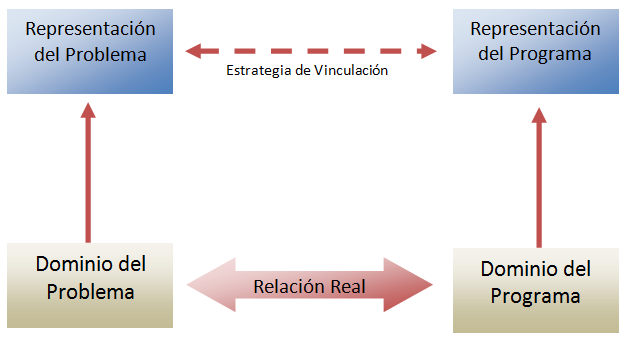
\includegraphics[scale= 0.50]{./dom.png}
\caption{Gráfico de Comprensión de Programas}
\end{figure} \label{captura1}

El inconveniente es que esta relación real es compleja de armar, por ende se puede bosquejar una aproximación mas accesible a través de los siguientes pasos: i) Elaborar una representación para el Dominio del Problema; ii)
Construir una representación del Dominio del Programa y iii) Elaborar un procedimiento de vinculación.
 
Para lograr con éxito los pasos antedichos se deben tener en cuenta conceptos muy importantes que son cimientos sobre los cuales esta sustentada la CP: los modelos cognitivos, la extracción de información, la interconexión de dominios y la visualización de software.

\section{Modelos Cognitivos}

Los \textit{Modelos Cognitivos} se refieren a las estrategias de estudio y las estructuras de información usadas por los programadores para comprender los programas. Estos modelos son importantes porque indican de que forma el programador comprende los sistemas y como incorpora nuevos conocimientos (aprende nuevos conceptos) \cite{MBPHRU10}.

Los modelos cognitivos abarcan 3 conceptos importantes: Conocimiento, un modelo mental y un proceso de asimilación \cite{MAS05}.

Existen 2 tipos de conocimientos uno es el conocimiento interno el cual se refiere al conocimiento que el programador ya posee antes de analizar el código del sistema de estudio. Por otro lado existe el conocimiento externo que representa un soporte de información externo que le brinda al programador nuevos conceptos. Los ejemplos mas comunes son la documentación del sistema, otros desarrolladores que conocen el dominio del problema, códigos de otros sistemas con similares características.

El concepto modelo mental hace referencia a representaciones mentales que el programador elabora en su mente al momento de estudiar el código del sistema. Estas representaciones mapean a distintas componentes del sistema. Algunos modelos construidos por los arquitectos del software como por ejemplo el \textit{Unified Modeling Language} UML, \textit{Entity Relationship} ER entre otros pueden verse como representaciones visuales de modelos mentales. 

Por último, el proceso de asimilación son las estrategias de aprendizaje que el programador usa para llevar adelante la comprensión de un programa. Los procesos de asimilación se pueden clasificar en tres grupos: Botton-up, Top-Down y distintas combinaciones de las anteriores(híbrida)\cite{MPOB03}.

El modelo de comprensión Botton-up indica que en primera instancia el código del sistema se lee por el desarrollador y luego el código se simplifica en un modelo mental, en pocas palabras se elabora una abstracción mental del código.

Por otro lado el modelo de comprensión top-down es una estrategia en donde primero el programador usa el conocimiento adquirido del dominio del problema para construir perspectivas del sistema en forma de modelo y luego estas perspectivas se vinculen con los distintos fragmentos del código.

Por ultimo el modelo híbrido que combina los dos conceptos mencionados top-down - bottom-up se adapta mucho mejor a los conocimientos que el programador posea durante el proceso de asimilación y con esto se logra mejores resultados.

Varios autores concluyen que estos conceptos conforman la base para encontrar la relación entre el dominio del problema y el dominio del programa \cite{TIE89,MPOB03}.

Para resumir sobre la temática de modelos cognitivos: el modelo mental es una representación mental que el programador tiene sobre el sistema. Si esta representación se la vincula con los conocimientos que el propio programador posee se logra un entendimiento completo del sistema como así también incrementa los conocimientos del programador. Con esto se deja en claro la importancia de modelos cognitivos en el proceso de entendimiento de los sistemas \cite{MBPHRU10}.

\section{Extracción de Información}

En la ingeniería del software existe una temática que se encarga de desarrollar/usar técnicas para la \textit{extracción de la información} en códigos de los sistemas, estas técnicas están catalogadas según el tipo de información que extraen.
Esta información puede ser: Estática o Dinámica, dependiendo de las necesidades del ingeniero de software o del equipo de trabajo. La principal diferencia que radica entre ambas técnicas es que las dinámicas requieren que el sistema se ejecute, mientras que las estáticas esto no es necesario.

La información estática esta contenida en el código fuente del sistema 
tipos, identificadores, procedimientos, y demás componentes visibles forman parte del código. Una estrategia para extraer la información estática consiste en utilizar técnicas tradicionales de compilación que extraigan los componentes del código deseados sin necesidad de ejecutar el programa.
%Para construir el analizador se suele utilizar una herramienta automatizada que lee una gramática y después genera el parser. En esta gramática asociada a un lenguaje particular se insertan acciones semánticas que formarán parte del parser generado.
Otra forma es usando grafo de llamadas a funciones en donde las aristas son funciones del programa de estudio y los arcos representan las llamadas entre dos funciones. A nivel conceptual es fácil de entender pero a veces la complejidad de los sistemas impiden una ágil realización sobre todo si los bloques de código tienen una complejidad temporal y espacial con cotas elevadas \cite{MBPHRU10}. Para la construcción de este grafo no se necesita ejecutar el programa.

Por otro lado la información dinámica se basa en elementos del programa presentes durante la ejecución del sistema. Para la extracción de este tipo de información se procede a bosquejar una técnica de instrumentación de código la cual consiste en insertar sentencias en el código sin modificar su semántica, así cuando el sistema se ejecute estas sentencias que contienen acciones se van a encargar de indicar que operaciones internas se llevaron a cabo para una determinada salida del programa.
La incorporación de estas sentencias debe realizarse con sumo cuidado y de forma estratégica para no alterar el flujo normal de ejecución.

Volviendo al objetivo principal que es aproximarse en la construcción de relación del dominio del problema con el dominio programa a través de representaciones esta requiere la extracción de información de ambos dominios.

La extracción de información del dominio del programa es una metodología sencilla de llevar a cabo por el hecho de que su extracción esta claramente marcada. El inconveniente radica en la extracción de la información perteneciente al dominio del problema, porque esta información es sensible a las características propias de la aplicación. Para encarar este inconveniente la ingeniería del software propone tomar las fuentes de información informal las cuales pueden estar presentes en el código por ejemplo: comentarios, literales string; o fuera del mismo: documentación, entrevistas con el cliente etc. Un vez que se extraen estos componentes se les puede aplicar alguna técnica de análisis de información informal para interpretar algunas las funcionalidades de los componentes del sistema.

Hasta aquí solo se ha mencionado estrategias de extracción información de los dominios del problema y del programa. Desafortunadamente el mapeo que relaciona la salida del sistema con los componentes que la integran queda a manos del programador y no abundan herramientas automatizadas que simplifiquen esta tarea.

\section{Estrategias de Interconexión de \\Dominios}

La \textit{Interconexión de Dominios} \cite{BRM10} tiene como principal objeto de estudio la transformación y vinculación de un dominio específico en otro dominio.
El punto importante es que cada componente de un dominio se vea reflejado en una o más componentes del otro y viceversa. 

Cuando se dice que relacionar el dominio del problema con el dominio del programa es importante ya que permite al desarrollador encontrar de forma mas ágil y rápida componentes en el software para una operación especifica. Esto facilidad impacta directamente en los tiempos dedicados a la evolución y al mantenimiento del software por el simple hecho de que se reduce la ardua tarea que tiene el programador de comprender el código.
Sin embargo solo se podrá destacar este impacto si el software de estudio es muy amplio y complejo.

%Los conceptos mencionados en los puntos anteriores como la visualización de software y la instrumentación de código forman la base para armar estrategias de interrelación de dominios.
A modo de ejemplo sobre interrelación de dominios, un caso es la transformación de un código fuente Dominio del Programa) en un Grafo de Llamadas a Funciones (Dominio de Grafos) como se mencionó en la sección anterior. Es importante aclarar que existe una amplia gama de transformaciones pero la más escasa y difícil de conseguir aquella que relaciona el Dominio del Problema con el Dominio del Programa.

Sin embargo actualmente existen técnicas recientemente elaboradas que conectan visualmente el dominio del problema y el dominio del programa usando la información estática y dinámica que se extrajo del sistema de estudio.

Una de las técnicas es \textit{Simultaneous Visualization Strategy} SVS, esta se encarga de mostrar los distintos componentes de un programa en plena ejecución, mediante distintas vistas, usando un inspector de sentencias, de esta manera se obtiene una visualización cuando el sistema se está ejecutando. Esta estrategia usa un esquema de instrumentación de código que se describió en párrafos precedentes, donde las acciones semánticas le van indicando a un visualizador la traza de invocaciones a funciones durante la ejecución del sistema \cite{BRM10,MPMR07}.

La otra estrategia se denomina \textit{Behavioral-Operational Relation Strategy} BORS, que a diferencia del SVS, espera a que termine la ejecución del sistema y luego la información recopilada por el instrumentador de código es procesada por BORS, entonces una abstracción gráfica del código ejecutado es devuelta por ejemplo como Árbol de Ejecución de Funciones. De esta forma se puede vincular mas claramente los conceptos del código capturados en tiempo de ejecución con la información asociada al dominio del problema \cite{BRM10,MPMR07}.

Existe también a nivel conceptual una técnica que combina ambas estrategias mencionadas llamada \textit{Simultaneous Visualization Strategy Improved} SVSI. Esta técnica disminuye los problemas que manifiestan tanto SVS como BORS y con ello se logra un mejor desempeño en cuanto a los resultados esperados \cite{BRM10,MPMR07}.

\section{Visualización de Software}

La \textit{Visualización del Software} es un pilar importante en la comprensión de programas, básicamente provee una o varias representaciones visuales (o vistas) de algún sistema particular. 

Existen distintos tipos de vistas, en si mismo, la primer vista de un sistema es el código en donde la información no esta tan clara para un desarrollador ajeno sobre todo si el software es grande y complicado. Es por eso que se necesita recurrir a otras vistas que representen una abstracción mas clara del sistema.
Las vistas poseen distintas características y para su construcción se requieren un conjunto de librerías gráficas. Dichas librerías son programas que simplifican la elaboración de las vistas y el diseñador de la visualización tiene la tarea de elegir que librería es la mas adecuada para la vista que desea construir. Las librerías gráficas mas conocidas son Jung, Prefuse, Graphviz y Cairo \cite{BRM10}. Las vistas cuando están bien construidas brindan una clara información del sistema y por ende facilita su comprensión. 

Los sistemas de visualización (SV) de software son herramientas útiles que se encargan de analizar los distintos módulos de un programa y generar vistas, dependiendo de la información que se desea visualizar existe una vista especifica \cite{MPMR07}. Cabe recordar que la información concebida en un sistema puede ser estática o dinámica.

Después de investigar distintos SV que actualmente existen: Myers, Price, Roman and Kenneth, Storey \cite{MBPHRU10}
en donde se concluye que la mayoría apuntan a capturar conceptos situados solo en el dominio del programa restando importancia al dominio del problema y a la relación entre ambos dominios. Debido a esta falencia Berón \cite{MBPHRU10} propone SV orientados a la CP ampliando aun mas los sistemas que hoy por hoy ya existen.

Para concluir se dice que la visualización de software orientada a la comprensión de programas tiene como principal desafío generar vistas que ayuden a relacionar el Dominio del Problema con el Dominio del Programa. 

\section{Comentarios}

Para resumir las ideas tratadas en este capítulo, comprender un programa se centra en la relación entre ambos dominios el del programa y del problema, como es demasiado complicado este vínculo, se llevan a cabo representaciones haciendo la \textit{extracción de información} correspondiente a cada dominio. Una vez construidas las representaciones de ambos dominios se procede a la elaboración de una estrategia de vinculación, el armado de esta estrategia se basa en los conceptos de \textit{interconexión de dominios}. Esta estrategia de vinculación ayuda al programador a entender con facilidad los programas ya que encuentra las partes del sistema que produjeron una determinada salida. La temática asociada a la \textit{Visualización del Software} indica que si se elaboran determinadas vistas se puede materializar gráficamente las representaciones de los dominios y la estrategia de vinculación (ver figura 2.1). Estas vistas ayudan a armar un puente cognitivo entre los aspectos del sistema y los conocimientos del programador, con esto se logra que el programador elabore una abstracción del sistema adecuada a su estructura mental.

Todos estos conceptos se deben tener en cuenta para uso/creación de Herramientas de Comprensión.
Las Herramientas de Comprensión son apropiadas para facilitar la comprensión de software ya que presenta diferentes perspectivas del sistema facilitando su análisis y su inspección.


%CAPITULO3=============================================================


\chapter{Análisis de Identificadores: Estado del Arte}

\lhead[]{CAPÍTULO 3. ANÁLISIS DE IDS: ESTADO DEL ARTE}

En el capítulo anterior se introdujo en el ámbito de comprensión de programas con las definiciones de los conceptos mas importantes. Este capítulo se centra en el estado del arte de técnicas que basan su análisis en los identificadores (ids) presentes en los códigos de los programas y también de algunas herramientas que implementan dichas técnicas.

\section{Introducción}

Los equipos de desarrollos de software frecuentemente enfocan todo su esfuerzo en el análisis, diseño, implementación y mantenimiento de los sistemas, restandole importancia a la documentación. Por lo tanto es común encontrar paquetes softwares carentes de documentación lo cual indica que la lectura de los códigos de los sistemas es la única manera de interpretarlos. Es necesaria la interpretación del sistema sobre todo en grandes equipos de desarrollo por el simple hecho de que un integrante del equipo puede tomar código ajeno para continuar con su desarrollo o realizar algún tipo de mantenimiento (Ver capítulo 2).

Teniendo en cuenta que los códigos de los sistemas crecen a partir de los nuevos requerimientos y el frecuente mantenimiento, esto implica que cada vez mas los sistemas se hacen mas complejos y difíciles de entenderlos. He aquí la importancia del uso de las herramientas de comprensión, con ellas se puede lograr un entendimiento ágil y facilitar las arduas tareas de interpretación de códigos.

Como se mencionó en el capítulo anterior la CP desarrolla métodos, técnicas y herramientas que facilitan al programador entender los programas.

La extracción de información estática es un aspecto importante de la CP (Capítulo 2) en donde se pueden aplicar técnicas de compilación conocidas para extraer información oculta detrás de los componentes visibles en los códigos de los programas sin necesidad de ejecutarlos.

%whats the name - Lawrie
Existen dos fuentes importantes de información que se encuentran dentro de los códigos de los programas una son los comentarios y la otra son los ids. Sin embargo cuando en el código no abundan los comentarios la única fuente son los ids.

%Uno de los componentes mas importantes presentes en los códigos de los sistemas que contienen información oculta son los identificadores (ids).

El la siguiente tabla se muestra un análisis léxico que se realizó sobre 2.7 millones de lineas de códigos escritos en lenguaje JAVA.\\

\begin{center}
   \begin{tabular}{| l | c | c | c | c | }
     \hline
     \textsf{Tipo} & \textsf{Cantidad} & \textsf{\%} & \textsf{Caracteres} & \textsf{\%} \\ \hline
     Palabras claves & 1321005 & 11.2 & 6367677 & 12.7 \\ \hline
     Delimitadores & 5477822 & 46.6 & 5477822 & 11.0 \\ \hline
     Operadores & 701607 & 6.0 & 889370 & 1.8 \\ \hline
     Literales & 378057 & 3.2 & 1520366 & 3.0 \\ \hline          
     \textbf{Identificadores} & 3886684 & 33.0 & \textbf{35723272} & \textbf{71.5} \\ \hline
     \textbf{Total} & \textbf{11765175} & \textbf{100.0} & \textbf{49978507} & \textbf{100.0} \\ \hline          
   \end{tabular}
\end{center}


Se ve claramente que mas de las dos terceras partes (71.5\%) de los caracteres en el código fuente forman parte de un id\cite{DFPM05,DMDJ13}. 

Por ende en el ámbito de CP los ids son una fuente importante de información que el lector del código o encargado de mantenimiento debe tener en cuenta. Utilizar una herramienta que analice los ids dando a conocer su significado ayuda a revelar esta información, mejora la comprensión, aumenta la productividad y agiliza el mantenimiento de los sistemas.

Por lo antedicho, construir herramientas de CP que se encargan de analizar ids en los códigos fuentes de los programas constituye un aporte importante al ámbito de CP. Antes de comenzar en la incursión de herramientas existentes que analizan ids, se detallan algunos conceptos claves relacionados a los ids.

\section{Conceptos claves}

\textit{“Un \textbf{Identificador (id)}: básicamente se define como una secuencia de letras, dígitos o caracteres especiales de cualquier longitud que sirve para identificar las entidades del programa (clases, funciones, variables, tipos estructurados, etc.)”}
 
Cada lenguaje tiene sus propias reglas que definen como pueden estar construidos los nombres de sus ids. Por lo general lenguajes como C y JAVA no esta permitido declarar ids que coincidan con palabras reservadas o que contengan algunos símbolos especiales (\$,\&,\#) a excepción de guiones(\_ ,$\--$).

Un id en un programa esta asociado a un concepto del programa. 

\begin{center}
\textsf{Identificador $\Leftrightarrow$ Concepto}
\end{center}

Dicho de otra manera un id es un representante de un concepto ubicado en el dominio del problema\cite{DFPM05,DMDJ13}.%mas biblografia

%whats the name - Lawrie
Para mejorar la CP se requiere que los nombres de los ids comuniquen de manera clara los conceptos que representan\cite{DFPM05,DLHD06,DCHD06}. Sin embargo esto no sucede frecuentemente. En la siguiente sección se menciona como el nombramiento de los ids impacta enormemente en la lectura comprensiva del código fuente.


\section{Nombramiento de Identificadores}

%Deißenbock and Pizka DFPM05
%Intro
Durante los desarrollos de los sistemas, las reglas de nombramiento de ids se enfocan más en el formato del código y en la documentación en lugar de enfocarse en el concepto que el id representa. Luego durante la etapa de mantenimiento del software la forma en la que los ids están nombrados no es muy tenida en cuenta para comprender el sistema.

\subsection{Clasificación}
Estudios realizados sobre 100 programadores\cite{DCHD06} sobre comprensión de ids indican que existen tres tipos principales de nombramiento (tomando como ejemplo el concepto \textsf{File System Input}): 

\begin{itemize}
\itemsep0em%reduce espacio
\item Palabras completas (\textsf{fileSystemInput}).
\item Abreviaciones (\textsf{flSysIpt}).
\item Una sola letra\footnote[1]{Este nombramiento lo llaman acrónimo algunos autores} (\textsf{fsi}). 
\end{itemize}

De mas esta decir que los nombres de los ids pueden estar compuestos por mas de una palabra como claramente se muestra arriba en los 2 primeros casos.

El estudio arrojó que las palabras completas son las mas comprendidas, sin embargo las estadísticas marcan en algunos casos que las abreviaciones que se ubican en segundo lugar no demuestran una diferencia notoria con respecto a las palabras completas\cite{DCHD06}.

A su vez los autores  Feild, Binkley, Lawrie \cite{FBL06,HDD06,DMDJ13} en los nombramientos que contienen mas de una palabra como es el caso de las \textit{palabras completas} y las \textit{abreviaciones} hacen 2 distinciones extras conocidas como \textit{hardwords} y \textit{softwords}.

Los \textit{hardwords} destacan la separación de cada palabra que compone el identificador a través de una marca específica; algunos ejemplos son: \textsf{fileSystem}\footnote[1]{Algunos autores lo llaman camel-case a este nombramiento} marca bien la separación de cada palabra con el uso de mayúscula entre las minúsculas o \textsf{fileSYSTEM} así también como utilizar un símbolo especial como es el caso del guion bajo \textsf{file\_system}. 

En cambio los \textit{softwords} no poseen ningún tipo de separador o marca que de indicios de las palabras que lo componen; por ejemplo: \textsf{textinput} o \textsf{TEXTINPUT} esta compuesta por \textsf{text} y por \textsf{input} sin tener una marca que destaque la separación.

%Si bien en el párrafo anterior se dio una taxonomía de como se clasifican los ids, en los ejemplos no se refleja como normalmente se nombra un id.
%Generalmente los programadores para reducir el esfuerzo de tipeo escriben los ids en forma abreviada compuestos por mas de una palabra, esto se lo conoce con el nombre de acrónimos. Para dar un ejemplo sobre esto: el id \textsf{fileSystem} los programadores lo suelen nombran como \textsf{flSys}, \textsf{fiStm}, \textsf{fl\_sys} u otras tantas posibles representaciones abreviadas.

%Caprile and Tonella state that “identifier names are one of the most important sources of information about program entities”\cite{BCPT00}

%Caprile and Tonella - Software entities are born and live with their names. \cite{BCPT99}

%================================
\subsection{Importancia del Nombramiento}
En la actualidad existen innumerables convenciones en cuanto al nombramiento sintáctico de los ids, alguna de ellas son:

\begin{itemize}
\itemsep0em%reduce espacio
\item En el caso de JAVA los nombres de los paquetes deben ser con minúscula (main.packed) y las clases con mayúscula en la primer letra de cada palabra que compone el nombre (MainClass).

\item En el caso de C\# las clases se nombran igual que JAVA pero los paquetes en cada nivel de nombre debe comenzar con mayúscula y resto minúscula (Main.Packed).
\end{itemize}

Esto indica que se concentra mas en los aspectos sintácticos del id y no tanto en los aspectos semánticos en lo que respecta al nombramiento. 

%Las investigaciones realizadas por Deissenboeck y Pizka \cite{DFPM05} a este problema parte de que cada nombre de id esta asociado a un concepto del dominio del problema y viceversa. 
%Mas formalmente se puede ver como una función biyectiva:

%\begin{center}
%\textsf{Nombre $\Leftrightarrow$ Concepto}
%\end{center} 

%En este contexto se dice que se logra un nombramiento conciso y consistente de ids.

\begin{figure}[t] %[h] para here [b] para bottom [t] para top
\centering
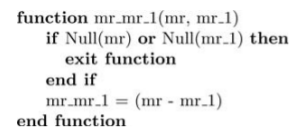
\includegraphics[scale= 0.70]{./idd_1.png}
\caption{Trozo de Código de un Sistema Comercial}
\label{captura2}
\end{figure} 

%Problema: de porque no existe un correcto nombramiento
Una evidencia fehaciente de la importancia en el nombramiento semántico son las técnicas que se aplican para protección de código, algunas de ellas se encargan de reemplazar los nombres originales de los ids por secuencias de caracteres aleatorios 
para reducir la comprensión, esta se conocen con el nombre de ofuscación de código. La ofuscación es común en los sistemas de índole comercial, en la figura \ref{captura2} se puede observar un ejemplo tomado de un caso real en donde la función \textsf{mr\_mr\_1} no parece complicada pero se desconoce la finalidad de su ejecución\cite{DFPM05}.

A su vez los programadores cuando programan restan importancia al correcto nombramiento semántico de los ids, existen tres razones destacadas que conllevan a esto:

\begin{enumerate}
\itemsep0em%reduce espacio
\item Los ids son escogidos por los desarrolladores y eluden el análisis automático.

\item Los desarrolladores tienen poco conocimiento de los nombres usados en los ids ubicados en otros sectores del código fuente.

\item Durante la evolución del sistema los nombres de los ids se mantienen y no adaptan sus nombres a las nuevas funcionalidades(o conceptos) que pueden tener.
\end{enumerate}

En este sentido el mal nombramiento de los ids se combate con la programación “menos egoísta” que consiste en hacer programas mas claros y entendibles para el futuro lector que no esta familiarizado. Para lograrlo se deben respetar dos reglas en cuanto al nombramiento\cite{DFPM05,DLHD06}:

%\noindent remueve la sangria!
\begin{framed}
\noindent \textbf{Nombramiento Conciso:} El nombre de un id es conciso si la semántica del nombre coincide exactamente con la semántica del concepto que el id representa.

\noindent \textbf{Nombramiento  Consistente:} Para cada id debe tener asociado si y solo si un único concepto.
\end{framed}

Un ejemplo de conciso es \textsf{output\_file\_name} que representa el concepto de `nombre de archivo de salida', distinto es \textsf{file\_name} no representa de forma semánticamente concisa el concepto mencionado.

%sinonimos y homonimos
Los propiedades que violan el nombramiento consistente en los ids son conocidos en el lenguaje natural con el nombre de sinónimos y homónimos. Los homónimos son palabras que pueden tener mas de un significado por ende el concepto al que esta asociado no esta muy claro (Ej: un id con el nombre `file' generalmente se asocia al concepto de archivo pero puede que se refiera a una estructura o a una fila de una tabla). Por otro lado los sinónimos indican que para un mismo concepto pueden tener asociados diferentes nombres (Ej: un id con el nombre `accountNumber' y otro `account' hacen referencia al mismo concepto `numero de cuenta bancaria'). Esta demostrado que la ausencia de nombramiento consistente tales como se menciono anteriormente hacen que se dificulte identificar con claridad los conceptos en el código y por ende aumenta los esfuerzos de comprensión del programa. 


Por lo tanto si los ids están nombrados de forma concisa (identificando bien al concepto) y la consistencia esta presente se pueden descubrir los conceptos que representan en el dominio del problema mas fácilmente y de esta manera agiliza la comprensión del código, aumenta la productividad, mejora la calidad durante la etapa de mantenimiento\cite{DFPM05,DLHD06}.%agregar mas bibliografia

Intuitivamente se concluye 	que mientras mejor nombrado estén los ids con respecto al concepto que representa, mayor es el impacto que tendrá en la interpretación del sistema\cite{DFPM05,DLHD06}.

En la practica es muy difícil mantener una consistencia global de nombres en los ids durante las etapas de desarrollo y mantenimiento del software, sobre todo si este es muy grande. Cada vez que un concepto se modifica el nombre del id asociado debe cambiar y adaptarse a la modificación pero esto no ocurre frecuentemente.

%solucion propuesta
Los autores Deissenboeck y Pizka\cite{DFPM05} proponen utilizar una herramienta que solucione los problemas de mal nombramiento planteados anteriormente, dado la dificultad que conlleva a la construcción de una herramienta totalmente automática que se encargue de nombrar correctamente los ids se elaboró una herramienta semi-automática que necesita la intervención del programador. Esta herramienta construye y mantiene un diccionario de ids a medida que el sistema se va desarrollando. En el ámbito de la ingeniería del software los diccionarios son muy útiles.

\begin{verse}
\textbf{Diccionarios de Datos:} Este concepto conocido también como `glosario de proyecto' se recomienda en los textos orientados a la administración de proyectos de software. Con los diccionarios se describe en forma clara todos los términos utilizados en los grandes sistemas de software y con esto se brinda una referencia completa a todos los participantes de un proyecto durante todo el ciclo de vida del producto.
\end{verse}

A continuación se describe la herramienta que ayuda al buen nombramiento de ids y mantiene la consistencia de nombres.

\begin{figure}[h] %[h] para here [b] para bottom [t] para top
\centering
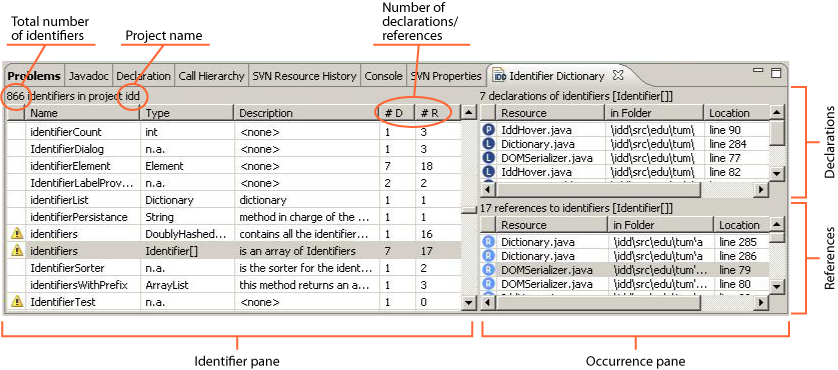
\includegraphics[scale= 0.50]{./idd_2.png}
\caption{Visualización de Identifier Dictionary}
\label{captura3}
\end{figure}
\pagebreak
\subsection{Herramienta: Identifier Dictionary}

La herramienta conocida con el nombre de \textit{Identifier Dictionary} (IDD)\footnote[1]{http://www4.informatik.tu-muenchen.de/\~{}ccsm/idd/index.html} básicamente actúa como un diccionario de datos que ayuda al desarrollador a mantener la consistencia de nombres en los ids de un proyecto JAVA. Es una base de datos que almacena información de los ids tales como el nombre, el tipo del objeto que identifica y una descripción comprensiva.

IDD ayuda a reducir la creación de nombres sinónimos y asiste a escoger un nombre adecuado para los ids siguiendo el patrón de nombres existentes. Aumenta la velocidad de comprensión del código en base a las descripciones de cada id. El equipo encargado de tareas de mantenimiento localiza un componente del domino del problema y luego su correspondiente id de manera ágil. Otro aporte que hace la herramienta es asegurar la calidad de los nombres(nombres concisos) de los ids con un esfuerzo moderado usando como ayuda la descripción comprensiva ubicada en la base de datos\cite{DFPM05,LFBEX07}.

Se implementó como extensión de la IDE Eclipse 3.1\footnote[2]{http://www.eclipse.org/jdt}. Se visualiza en el panel de las vistas de la IDE y consiste de tres secciones (Figura \ref{captura3}):

\begin{figure}[t] %[h] para here [b] para bottom [t] para top
\centering
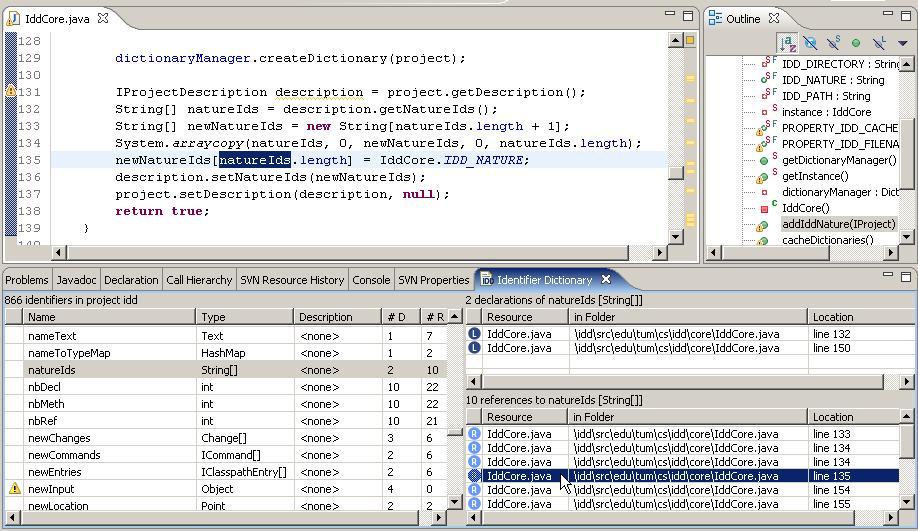
\includegraphics[scale= 0.40]{./idd_3.png}
\caption{Visualización de Identifier Dictionary}
\label{captura4}
\end{figure} 

\begin{itemize}
\itemsep0em%reduce espacio
\item Una tabla con información de los ids en el proyecto: nombre, tipo, descripción, cantidad de declaraciones y cantidad de referencias. (Identifier pane).
\item Una lista de Ids declarados en el proyecto (Ocurrence pane).
\item Una lista de referencias de los ids en el proyecto (Ocurrence pane).
\end{itemize}

Mientras se realiza el desarrollo del código la herramienta asiste al programador a llevar un buen nombramiento en los ids a través de las siguientes características:

\textbf{Navegación en el código fuente:} Si se selecciona un id en la tabla de ids (izquierda), la parte derecha mostrará las declaraciones y las referencias de ese id mostrando en las columnas de la derecha la ubicación exacta en donde se encuentra cada declaración y referencia(Figura \ref{captura4}).


%\begin{figure}[h] %[h] para here [b] para bottom [t] para top
%\centering
%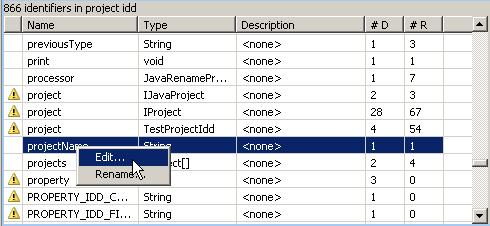
\includegraphics[scale= 0.55]{./idd_4.png}
%\caption{Visualización de Identifier Dictionary}
%\label{captura5}
%\end{figure}
%
%\textbf{Guardar descripción:} Botón derecho en el panel de ids y luego en edit. Permite agregar una descripción comprensiva (Figura \ref{captura5}).

%\begin{figure}[h] %[h] para here [b] para bottom [t] para top
%\centering
%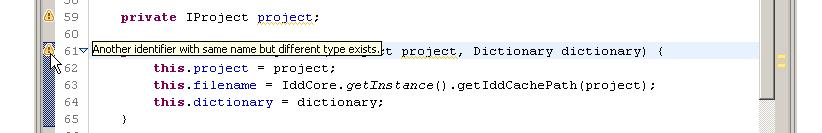
\includegraphics[scale= 0.55]{./idd_5.png}
%\caption{Visualización de Identifier Dictionary}
%\label{captura6}
%\end{figure}
\begin{figure}[t] %[h] para here [b] para bottom [t] para top
\centering
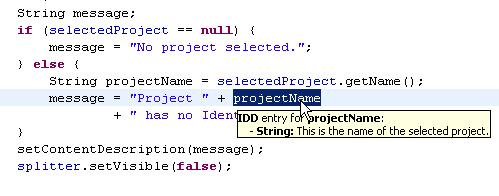
\includegraphics[scale= 0.80]{./idd_7.png}
\caption{Visualización de Identifier Dictionary}
\label{captura8}
\end{figure}

\textbf{Advertencias(warnings):} Mientras se realiza la colecta de ids los iconos de advertencia indican potenciales problemas en el nombramiento.  Los dos tipos de mensajes que se muestran son: dos ids con el mismo nombre pero distinto tipos y el id es declarado pero no referenciado\footnote[1]{Similar a los warnings de Eclipse}.


%\begin{figure}[h] %[h] para here [b] para bottom [t] para top
%\centering
%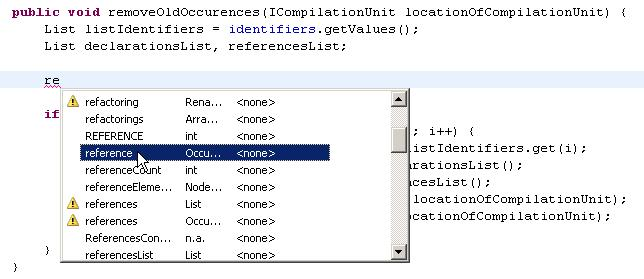
\includegraphics[scale= 0.55]{./idd_6.png}
%\caption{Visualización de Identifier Dictionary}
%\label{captura7}
%\end{figure}

\textbf{Mensajes pop-up:} Se puede visualizar información tales como la descripción del id posicionando el cursor sobre el id en el código fuente mientra se esta programando(Figura \ref{captura8}).

\textbf{Auto-completar nombres:} Las IDE actuales proveen la función de auto-completar. Sin embargo esta funcionalidad falla cuando los nombres de los ids no están declarados dentro del alcance actual de edición. El plugin IDD a la hora de auto-completar no tiene en cuenta el alcance desde el lugar que se esta editando, ademas de considerar el nombre del id también se considera el tipo.

%\begin{figure}[h] %[h] para here [b] para bottom [t] para top
%\centering
%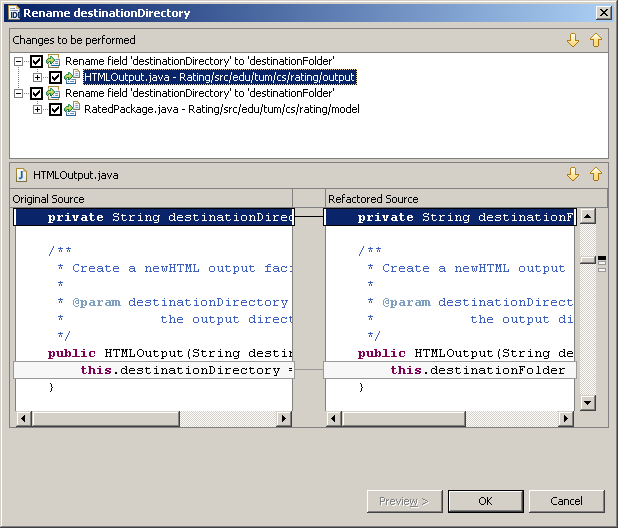
\includegraphics[scale= 0.55]{./idd_8.png}
%\caption{Visualización de Identifier Dictionary}
%\label{captura9}
%\end{figure}

\textbf{Renombre global de ids:} Esta función permite renombrar cualquier id generando una vista previa y validando el nombre de los ids a medida que sistema va evolucionando. De esta forma se preserva la consistencia global de nombres.

La herramienta IDD trabaja internamente con un colector de ids que esta acoplado al proceso de compilación del proyecto(Build Proyect) de Eclipse. Los ids se van recaudando a medida que el programa se va compilando. Los nombres, el tipo, la descripción se van guardando en un archivo XML. También se puede exportar en un archivo en formato HTML el cual permite una lectura más clara de los ids con toda información asociada\cite{DFPM05}.


%%=========Lawrie

La herramienta colabora en mejorar el nombramiento de los ids con un esfuerzo moderado como se describió antes, sin embargo otros autores\cite{LFBEX07,DLHD06} determinan que los esfuerzos son moderados solo para sistemas que se empiezan a programar desde el comienzo y no con sistemas ya existentes.

Para concluir con esta sección la buena calidad en el nombramiento de los ids descripta anteriormente no solo mejora el entendimiento del código sino que también facilita la construcción herramientas que ejecuten técnicas de regresión. Algunas técnicas traducen los nombres de los ids a palabras más completas en lenguaje natural y de esta manera facilitar el entendimiento de desarrolladores no tan expertos. En la sección siguiente se dan a conocer casos que utilizan estas técnicas de regresión.

%%=====================================
\pagebreak
\section{Traducción de Identificadores}

\subsection{Introducción}

Los lectores de códigos de programas tienen inconvenientes para entender el propósito de los ids y deben invertir tiempo en analizar el significado de su presencia. Estrategias automáticas dedicadas a facilitar este análisis son bienvenidas en el contexto de la CP.

La literatura correspondiente a estrategias de análisis de ids indican que los ids ocultan información relevante del domino del problema detrás de sus abreviaturas\cite{EHPV09,LFBEX07}. 

\subsection{Conceptos y Desafíos observados}

Una manera de desplegar la información oculta detrás de los ids es intentar convertir estas abreviaturas en palabras completas del lenguaje natural. Por ende el foco del análisis de los ids se basa en la traducción de palabras abreviadas a palabras completas.

El proceso automático que se lleva a cabo para realizar la traducción de ids consta de dos pasos\cite{LFBEX07}:

\begin{enumerate}
\itemsep0em%reduce espacio
\item \textbf{División:} Separar el id en las palabras que lo componen usando algún separador especial\footnote[1]{Siempre y cuando el id contenga más de una palabra.}. (Ejemplo: \textsf{flSys} $\Rightarrow$ \textsf{fl-sys}).

\item \textbf{Expansión:} Expandir las abreviaciones que resultaron como producto del paso anterior. (Ejemplo: \textsf{fl-sys} $\Rightarrow$ \textsf{file system}).
\end{enumerate}

Cabe mencionar que el ejemplo mostrado en ambos pasos corresponde a un caso de \textit{hardword} (ver sección anterior) en donde la separación de las palabras es destacada. Sin embargo la dificultad se presenta en los \textit{softwords}(ver sección anterior) ya que la división no esta marcada(Ejemplo: \textsf{hashtable} $\Rightarrow$ \textsf{hash-table}). Existen también casos híbridos (Ejemplo: \textsf{hashtable\_entry}). En este caso el id tiene una marca de separación (guión bajo) con dos hardwords \textsf{hashtable} y \textsf{entry}. A su vez el hardword \textsf{hashtable} posee dos softwords \textsf{hash} y \textsf{table}, mientras que \textsf{entry} es un hardword compuesto por un solo softword. 

%noindent - Elimina sangria
\begin{framed}
\noindent El objetivo primordial del análisis de ids es detectar los casos de softword luego proceder a separar las palabras abreviadas que la componen para posteriormente realizar la expansión\cite{FBL06,LFBEX07}.  
\end{framed}

Para llevar a cabo la tarea de traducción de ids es necesario recurrir a fuentes de palabras en lenguaje natural (inglés en este caso). Existen 2 tipos de fuentes, dentro del mismo código extrayendo palabras presentes en comentarios, literales y documentación. La otra fuente se encuentra fuera del programa consultando diccionarios o listas de palabras predefinidas.\\\\Algunos inconvenientes que se presentan cuando se desarrollan herramientas que traduzcan ids:

\begin{description}
\itemsep0em%reduceenglish espacio
\item[Dificultad para armar diccionarios apropiados:]  La mayoría de los diccionarios en Inglés se usan para corregir la ortografía. Las palabras que incluyen son sustantivos propios, abreviaciones, contracciones\footnote[1]{Palabras en ingles que llevan apostrofes ej: let's.} y demás palabras que puedan aparecer en un software. Sin embargo la inclusión de muchas palabras genera que una simple abreviación ($char,tab,id$) se trate como una palabra expandida y no se expanda. Por el contrario si contiene pocas palabras, la expansión se realiza mas frecuente de lo normal.
% lo ideal es disponer de un diccionario con palabras que incluyan solo palabras adecuadas al ámbito de la ciencias de la computación pero lamentablemente esto no esta disponible.

\item[Las abreviaciones poseen muchos candidatos a expandir:] Es complicado para un id abreviado con \textsf{def} determinar con precisión cual es la mejor traducción entre tantos candidatos \textsf{definition, default, defect}. Otra observación hecha es que mientras mas corta es la abreviación mas candidatos posee y lo que mas frustra es que la mayoría de los ids poseen entre 1 y 3 caracteres, el mas común es \textsf{i} que generalmente es \textsf{integer} pero podrían ser otros \textsf{interface, interrupt},etc. Se requieren procesos inteligentes para solucionarlo.

\item[El tipo de la abreviación afecta el numero de candidatos:] Si la abreviatura se mira como prefijo tiene menos candidatos a traducirse, un ejemplo es \textsf{str} el cual tiene \textsf{string, stream} en cambio si las letras de la abreviatura forman parte de la palabra tiene mas posibilidades \textsf{substring, store, september, saturn}.
\end{description}


Las palabras abreviadas usadas en los ids dependen mucho de la idiosincrasia del programador. Por lo tanto construir herramientas automáticas que analicen ids representa un verdadero desafío en el área de CP.

En las próximas 2 secciones se detallan algoritmos encargados de la división de ids, y en la secciones subsiguientes se describen algoritmos de expansión.

%Se puede usar técnicas de recuperación de información para mejorar el procedimiento de traducción.

%greedy - samurai 
\subsection{Algoritmo de División: Greedy}

El algoritmo de greedy elaborado por Lawrie, Feild, Binkley\cite{FBL06,LFBEX07} es sencillo y emplea tres listas:
\begin{description}
\itemsep0em%reduce espacio
\item[Palabras de diccionarios:] Contiene palabras de diccionarios públicos sumado a las palabras del comando de Linux \textsf{ispell} que corrobora ortografía en la linea de comandos.

\item[Abreviaciones conocidas:] La lista se arma con abreviaciones extraídas de distintos programas y de autores expertos. Se incluyen abreviaciones comunes (ej: \textsf{alt} $\rightarrow$ \textsf{altitude}) y abreviaciones de programación \mbox{(ej: \textsf{txt} $\rightarrow$ \textsf{text}).}

\item[Palabras excluyentes(stop list):] Posee palabras que son irrelevantes para realizar la división de los ids incluye palabras claves(ej: \texttt{while}), ids predefinidos(ej: \texttt{NULL}), nombres y funciones de librerías (ej: \texttt{strcpy},\texttt{errno}), y todos los ids que puedan tener un solo caracter. Esta lista es muy grande.
\end{description}

El algoritmo de greedy procede de la siguiente manera, el id que recibe como entrada primero se divide en las hardwords que lo componen(ej: \textsf{file\_txt} en \textsf{fileinput} y \textsf{txt}), cada hardword resultante que este en alguna lista antedicha se considera un solo softword. Si algún hardword no está en alguna lista se considera como múltiples softwords que necesitan subdividirse(ej: \textsf{fileinput} en \textsf{file} y \textsf{input}). La búsqueda en esos softwords toma el prefijo y el sufijo mas largo presente en alguna lista. Por un lado se ejecuta un proceso encargado de los prefijos, este empieza mirando toda la palabra por completo y se van extrayendo caracteres del final hasta encontrar el prefijo mas largo(o no haya mas caracteres). De manera simétrica, otro proceso encargado de los sufijos, extrae caracteres de la primera posición hasta encontrar el sufijo mas largo presente en alguna lista. Hasta que no se vacíe el string analizado ambas búsquedas se llaman recursivamente por los caracteres restantes. De esta manera se obtiene un alto ratio de división. Los softwords resultantes se separan con una marca\cite{FBL06,LFBEX07}.

\subsection{Algoritmo de División: Samurai}

Esta técnica pensada por Eric Enslen, Emily Hill, Lori Pollock, Vijay-Shanker\cite{EHPV09} divide a los ids en secuencias de palabras al igual que Greedy con la diferencia que la división es mas efectiva. La estrategia utiliza información presente en el código para llevar a cabo el objetivo. Esto permite que no sea necesario utilizar diccionarios predefinidos y las palabras que se obtienen producto de la división no están limitadas por el contenido de estos diccionarios. De esta manera la técnica va evolucionando con el tiempo a medida que aparezcan nuevas tecnologías y que nuevas palabras se incorporen al vocabulario de los programadores.

El algoritmo selecciona la partición mas adecuada en los ids multi-palabra\footnote[1]{Que posee mas de una palabra.} en base a una función de puntuación (scoring). Esta función utiliza información que se recauda extrayendo las frecuencias de aparición de palabras dentro del código fuente. Estas palabras pueden estar contenidas en comentarios, literales strings y documentación.

Esta estrategia de separación esta inspirada en un técnica de expansión de abreviaturas AMAP\cite{EZH08} que se presenta en las próximas secciones.

La técnica Samurai según el autor\cite{EHPV09} no solo divide los ids sino que también aquellos que aparezcan en los comentarios y en los literales strings. Esto ocurre porque el objetivo es mas amplio y no consiste en solo dividir ids. Por esta razón nombra al parámetro de entrada del algoritmo como \textit{token} y no \mbox{simplemente id.}

El algoritmo se encarga de extraer información respecto a la frecuencia de tokens en el código fuente y luego se construyen dos tablas de frecuencia de tokens. 

Para la construcción de una de las tablas primero se ejecuta el algoritmo que extrae del código fuente todos los tokens del tipo hardword. Estos tokens son agregados en la \textit{tabla de frecuencias específicas}, donde una entrada de la tabla corresponde al listado de tokens extraídos del programa actual bajo análisis (cada token es único en la tabla) y la otra entrada corresponde al numero de ocurrencia de cada token. Por otro lado existe la \textit{tabla de frecuencias globales} que contiene las mismas dos columnas que la tabla anterior, tokens y sus frecuencias pero en este caso la información es recolectada de distintos programas de gran envergadura. Durante el proceso de división del token, Samurai ejecuta la función de scoring que se basa en la información de ambas tablas antedichas\cite{EHPV09}.

\begin{figure}[h] %[h] para here [b] para bottom [t] para top
\centering
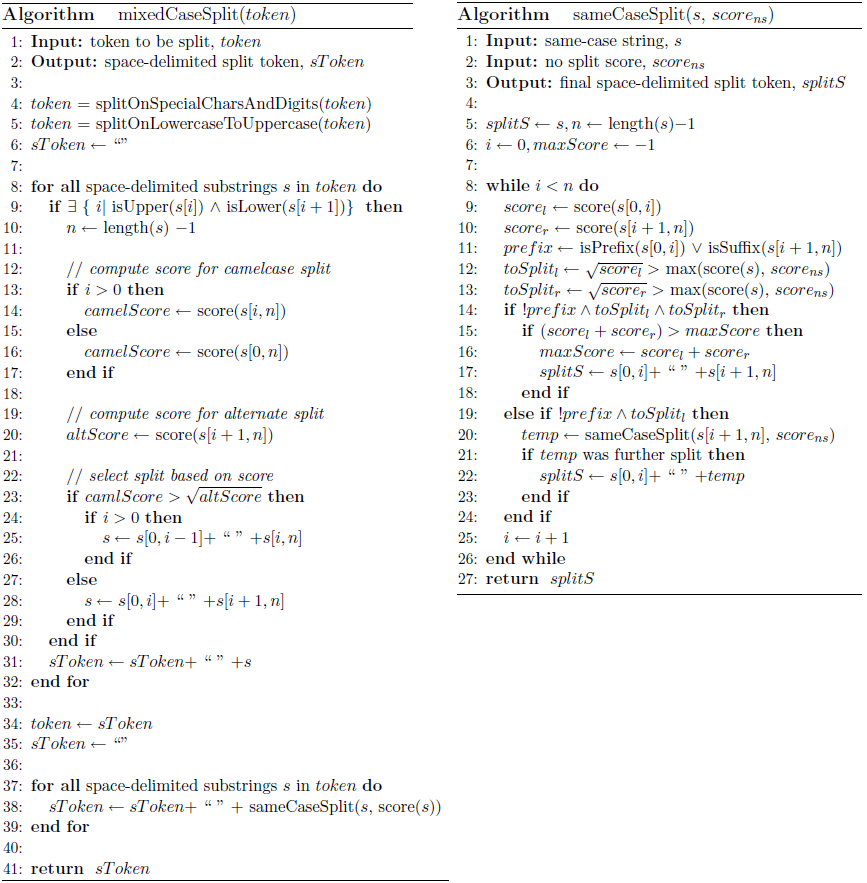
\includegraphics[scale=0.53]{./sam_1.png}
\caption{Algoritmos mixedCaseSplit y sameCaseSplit}
\label{sam1}
\end{figure}

%aclarar que puede recivir distintos tipos de ids ademas de los ya mencionados
El algoritmo ejecuta dos rutinas \textit{mixedCaseSplit} y después \mbox{\textit{sameCaseSplit}} (figura \ref{sam1}). La primera básicamente se encarga de dividir los hardwords (palabras que poseen guion bajo o son del tipo camel-case), luego cada una de las palabras obtenidas son pasadas a la segunda rutina para continuar con el análisis\cite{EHPV09}.

La rutina \textit{mixedCaseSplit} primero particiona usando dos funciones(líneas 4 y 5) \textit{splitOnSpecialCharsAndDigits} que reemplaza todos los posibles caracteres especiales por espacio en blanco y luego \mbox{\textit{splitOnLowercaseToUppercase}} de la misma forma que la anterior agrega un blanco entre dos caracteres que sea una minúscula seguido por una mayúscula. En este punto solo quedan tokens de la forma softword o que contengan una mayúscula seguido de minúscula (Ejemplos: \textsf{List, ASTVisitor, GPSstate, state, finalstate, MAX}).

Los casos de softword(\textsf{finalstate}, \textsf{MAX}) van directo a la rutina \mbox{\textit{sameCaseSplit}}. El resto del tipo mayúscula seguido de minúscula continua con el proceso de división para determinar cual es la separación de palabras mas adecuada utilizando la función de scoring(líneas 13-30). Son dos opciones que se pueden determinar en este punto: a) que la separación se realice entre el cambio de mayúscula y minúscula (ejemplo: \textsf{GPS state}) o b) que se a haga antes de la primer mayúscula siguiendo con la filosofía camel-case (ejemplo: \textsf{GP Sstate}). Aquella que tenga el puntaje (score) mas alto entre las dos será por la cual se decida, luego las partes resultantes son enviadas a \textit{sameCaseSplit}\cite{EHPV09}.

La próxima rutina \textit{sameCaseSplit} recibe como entrada un substring \textit{s}, el cual puede tener tres tipos de variantes: a) todos los caracteres en minúsculas o b) todos con mayúsculas o c) el primer caracter con mayúscula seguido por todas minúsculas(\textsf{Visitor}). La rutina primero examina cada punto posible de división en \textit{s} dividiendo en \textit{score(left)} y \textit{score(right)} respectivamente(línea 9 y 10). La decisión de cual es la mejor división se basa en a) substrings que no tengan prefijos o sufijos ordinarios\footnote[1]{Listas de prefijos y sufijos http://www.cis.udel.edu/˜enslen/samurai).}(línea 11) y b) el puntaje de la división elegida sobresalga del resto(líneas 12-14). 

%una sola division no se llama recursivamente (!prefix ^ toSplitl ^ toSplitr)
Para esclarecer este punto cada partición (izquierda o derecha) obtenida se calcula el score y luego este es comparado con el puntaje de la palabra original ($score_{ns}$ score original) y el puntaje de la palabra actual ($score(s)$). En un principio ambas son iguales pero a medida que avanza la recursión $score(s)$ varia con respecto a $score_{ns}$ (líneas 12 y 13).
%agregar ejemplos gráficos etc.

%si se cumple solo la parte izquierda se llama recursivamente (!prefix ^ toSplitl)
En caso de que solo se cumpla el ítem (a)(no tengan prefijos y sufijos ordinarios) se considera que la parte izquierda es un candidato y la cadena de la parte derecha se invoca recursivamente de nuevo con la rutina porque podría seguir dividiéndose en mas partes (línea 20).

Si la parte derecha se termina dividiendo, luego entre la izquierda y la derecha también. Sin embargo en caso que la parte derecha no se divida tampoco se debería separar entre ambas partes(el \textsf{if} de la linea 21 controla esto). Los análisis de datos\cite{EHPV09} indican que no se debe separar la actual posición en base solo a la evidencia en la izquierda ya que puede ser erróneo, un caso conocido erróneo es \textsf{string ified}). 

La ejecución recursiva de samurai para la cadena \textsf{nonnegativedecimaltype} se ejecuta correctamente y divide la cadena \textsf{nonnegative decimal type}\cite{EHPV09}.

Un problema son las palabras de pocos caracteres, porque tienen mucha aparición en los códigos y la cota de score es mas alta que las palabras mas largas. Por esta razón la raíz cuadrada se coloca en el resultado de score antes de comparar(línea 12 y 13), sino la división frecuentemente seria errónea, un ejemplo de esto es \textsf{per formed}.\\

\noindent \textbf{Función de Scoring}

Para que la técnica samurai pueda llevar a cabo la tarea de separación de ids se necesita la función de scoring. Como bien se dijo anteriormente esta función participa en 2 decisiones claves durante el proceso de división:

\begin{itemize}
\itemsep0em%reduce espacio
\item En la rutina \textit{mixedCaseSplit} para determinar si el la división del id es un caso de camel-case o no.

\item En la rutina \textit{sameCaseSplit} para puntuar las diferentes particiones de substrings y elegir la mejor separación.
\end{itemize}

Dado un string \textbf{s}, la función \textit{score(s)} indica la frecuencia de aparición de \textbf{s} en el programa bajo análisis y también la frecuencia en un conjunto grande de programas predefinidos. La formula es la siguiente:

\begin{center}
$Freq(s,p) + globalFreq(s) / \log_{10}(AllStrsFreq(p))$
\end{center}

Donde \textbf{p} es el programa de estudio, $Freq(s,p)$ es la frecuencia de ocurrencia de \textbf{s} en \textbf{p}. $AllStrsFreq(p)$ es la frecuencia total de todos los strings en el programa \textbf{p}. $globalFreq(s)$ es la frecuencia de aparición de \textbf{s} en una gran conjunto de programas tomados como muestras\footnote[1]{Estos programas son alrededor de 9000 y están escritos en JAVA}\cite{EHPV09}.

\pagebreak
\subsection{Algoritmo de Expansión Básico}
%noindent elimina sangria
%\noindent \textbf{Algoritmo 1}

El algoritmo de expansión de abreviaturas ideado por Lawrie, Feild, Binkley(mismos autores que la técnica de separación Greedy)\cite{LFBEX07, EZH08} trabaja con cuatro listas para realizar su tarea:

\begin{itemize}
\itemsep0em%reduce espacio
\item Una lista de palabras (en lenguaje natural) que se extraen del código.
\item Una lista de frases (en lenguaje natural) presentes también en el código.
\item Una lista de palabras irrelevantes (stop list).
\item Una lista de palabras de un diccionario en inglés.
\end{itemize}

La primer lista se confecciona de la siguiente manera, para cada función \textit{f} dentro del código se crea una lista de palabras que se extraen de los comentarios que están antes (comentarios JAVA Doc) o dentro de la función \textit{f}. También se incorporan los ids del tipo hardword(si existen) dentro del alcance local de \textit{f}. La lista de frases se arma utilizando una herramienta que las extrae, el principal recurso son los comentarios y los ids multi-palabras. En este punto se construye un acrónimo\footnote[1]{Abreviación formada por las primeras letras de cada palabra en una frase, gif: Graphics Interchange Format.} con las palabras de alguna frase, si ese acrónimo coincide con alguno de los ids extraídos, entonces esa frase se considera como potencial expansión (Ejemplo: la frase \textsf{file status exists} es una expansión posible en el id \textsf{fs\_exists}).

Una vez que las listas de palabras y frases potenciales se confeccionan, la expansión comienza. Este proceso conlleva dos etapas, primero se chequean las listas con palabras extraídas del código y de los comentarios, en caso de no tener éxito la búsqueda continúa con el diccionario compuesto con palabras en inglés como último recurso.

Las palabras en la lista de palabras irrelevantes(stop-list)\footnote[2]{Esta lista se usa con la misma política que el algoritmo Greedy.} incluyen artículos (the, an, etc.) y palabras reservadas del lenguaje de programación que se este utilizando (\textsf{while, for, if,} etc.). El significado de estas palabras no aporta información importante en la comprensión del código y son fácilmente reconocidas por los ingenieros del software.

%al igual que samurai stop list y steming usa tecnicas de ir - completar si es necesario

Esta técnica de expansión descripta solo retorna expansiones potenciales si cada una de ellas es única para una determinada abreviatura y en caso contrario no retorna nada. En este sentido como trabajo futuro se plantea la posibilidad de escoger de forma automática un sola expansión entre múltiples posibilidades para una abreviatura\cite{LFBEX07,EZH08}.

\subsection{Algoritmo de Expansión AMAP}
%noindent elimina sangria
%\noindent \textbf{\\Algoritmo 2}

El algoritmo de expansión de abreviaturas que construyó Emily Hill, Zachary Fry, Haley Boyd\cite{EZH08} conocido como \textit{Automatically Mining Abbreviation Expansions in Programs} (AMAP) ademas de buscar potenciales expansiones al igual que el algoritmo anterior, también se encarga de seleccionar la que mejor se ajusta en caso de que haya mas de un resultado posible.

Una mejora destacable con respecto al algoritmo previo es que no se necesita un diccionario con palabras en lenguaje natural. Los diccionarios (en inglés) incluyen demasiadas palabras e implica disponer de un gran almacenamiento. 

Las fuentes de palabras que se utilizan son una lista de abreviaciones comunes que se obtienen automáticamente desde distintos programas y puede a su vez incorporar palabras en forma personalizada. La lista palabras irrelevantes (stop-list) y la de contracciones más comunes se arman manualmente.

Para agilizar la lectura se asigna el nombre de “palabras abreviadas” aquellas que se desean expandir y “palabras largas” a las palabras normales que no están abreviadas.

La técnica automatizada busca palabras largas candidatas para una palabra abreviada dentro del código con la misma filosofía que se usa en la construcción de una tabla de símbolos en un compilador.

Se comienza con el alcance estático mas cercano donde se examinan sentencias vecinas a la palabra abreviada. Luego gradualmente el alcance estático crece para incluir métodos, comentarios de métodos, y los comentarios de la clase. Si la técnica no encuentra una palabra larga adecuada para una determinada palabra abreviada, la búsqueda continua mirando todo el programa y finalmente en JAVA SE 1.5. 

Los autores asumen que una palabra abreviada esta asociada a una sola palabra larga dentro de un método. Es inusual que dentro de un método una palabra abreviada posea mas de una expansión posible. En caso de que esto se cumpla se puede cambiar la asunción y estipular que una palabra abreviada solo tiene una sola expansión posible dentro de los bloques o achicando aun más solo dentro de las sentencias de código.


A continuación se explican los siguientes ítems: 1) Como se realiza la búsqueda para encontrar palabras largas candidatas dentro de un método. 2) Como se buscan nuevas palabras si el alcance local del método no es suficiente. 3) Como se elije entre varias opciones posibles cual es la mejor expansión.

Comenzando por el item 1, la búsqueda de las palabras largas contiene dos algoritmos, uno que recibe como entrada palabras abreviadas compuestas por una sola palabra(singulares) y el otro algoritmo se encarga de procesar multi-palabras.\\

\noindent \textbf{Búsqueda por Palabras Singulares\\}

El primer paso para buscar palabras largas consiste en construir una expresión regular con un patrón de búsqueda.  Este patrón se encarga de seleccionar las palabras largas que coincidan con las letras de la palabra abreviada.

La expresión regular se construye a partir de la palabra abreviada, a continuación se detalla como se arman los patrones: \\

\begin{description}
\itemsep0em%reduce espacio
\item[Patrón prefijo:] Se construye colocando la palabra abreviada ($sf$) seguida da la expresión regular [a-z]+. Las palabras que coinciden si o si deberán comenzar con $sf$. Finalmente la expresión regular queda: $sf$[a-z]+.

\item[Patrón compuesto por letras:]  La expresión regular se construye insertando [a-z]* después de cada letra de la palabra abreviada ($sf$). Si $sf=c_{1},c_{2},c_{3},..,c_{n}$, donde $n$ es la longitud de la palabra abreviada. El patrón queda: $c_{1}$[a-z]*$c_{2}$[a-z]*$c_{3}$[a-z]*..$c_{n}$.
\end{description}


\begin{figure}[h] %[h] para here [b] para bottom [t] para top
\centering
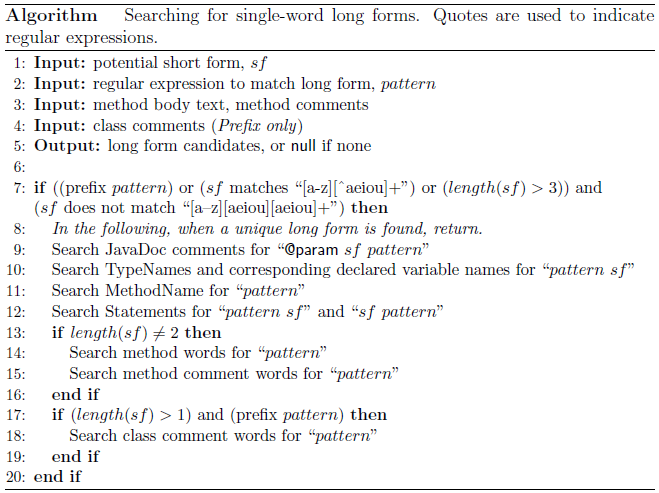
\includegraphics[scale=0.7]{./exp_1.png}
\caption{Algoritmo de Expansión de una sola Palabra.}
\label{exp1}
\end{figure}


En la figura \ref{exp1} se presenta un algoritmo\cite{EZH08} con un enfoque de búsqueda de palabras largas basada en abreviaturas compuestas por una sola palabra. Con el \textsf{if} de la línea 6 se impide básicamente dos cosas: que no se busquen palabras largas improbables de coincidir con la palabra abreviada pasada como entrada y que no se procesen palabras abreviadas con muchas vocales consecutivas. 

Esta comprobado que la mayoría de las palabras abreviadas con vocales consecutivas se expanden como multi-palabras (ej: \textsf{gui} $\rightarrow$ \textsf{graphical user interface}, \textsf{ioe} $\rightarrow$ \textsf{invalid object exception}) por ende de estos casos se encarga el algoritmo de la próxima sección.

En este algoritmo los autores determinaron que el \textit{patrón compuesto por letras} no se usara. Este patrón es muy flexible y se eligen palabras largas incorrectas(ej de casos incorrectos: \textsf{lang} $\rightarrow$ \textsf{loading}, \textsf{br} $\rightarrow$ \textsf{bar}, \textsf{mtc} $\rightarrow$ \textsf{matching}).

En las líneas 7-19 se describe el proceso de búsqueda. Si alguna de las sentencias de búsqueda encuentran un sola palabra larga candidata, el algoritmo finaliza y retorna el resultado. En la línea 8 se busca usando la palabra abreviada ($sf$) y el patrón dentro del comentario Java Doc en el método correspondiente. Si falla en la línea 9 se busca en los nombres de los tipos ubicados en las variables declaradas. Si no tiene éxito sigue en la línea 10 con el nombre del método. En caso de seguir sin resultado se continua en la línea 11 con distintas variantes del patrón en las sentencias. En la figura \ref{exp3} se pueden observar los distintos casos que se describieron.

Si la ejecución continua, la línea 12 se restringe la búsqueda por palabras que tengan al menos 3 caracteres ya que generalmente aquellas con 2 tienden a ser multi-palabras (ej: \textsf{fl $\rightarrow$ file system} / ver próxima sección). Luego en las líneas 13-14 se busca con el patrón en palabras del método y palabras de comentarios dentro del método.

\begin{figure}[h] %[h] para here [b] para bottom [t] para top
\centering
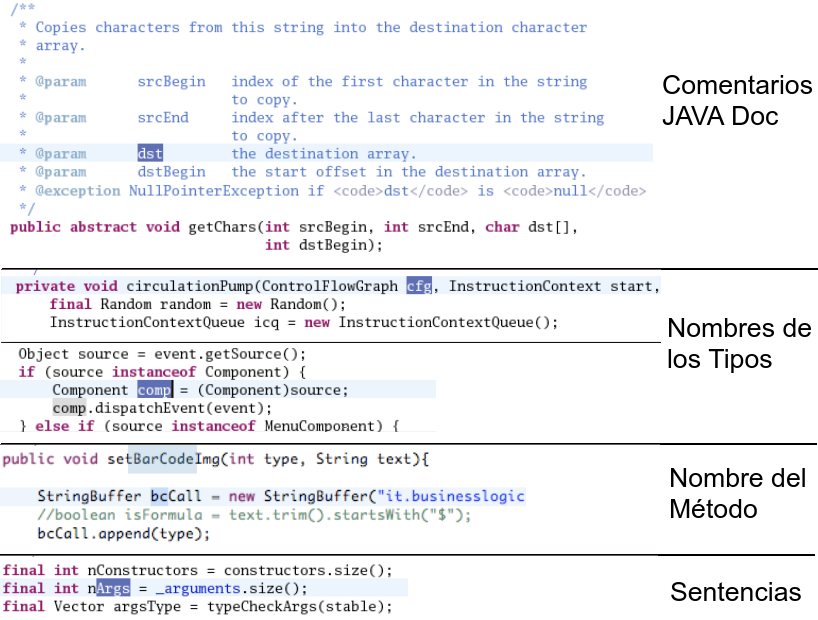
\includegraphics[scale=0.7]{./exp_3.png}
\caption{Ejemplos de trozos de Código.}
\label{exp3}
\end{figure}

Para finalizar en la línea 17 si la palabra abreviada es mas larga que un solo caracter y el patrón prefijo coincide, se comienza la búsqueda usando el patrón en los comentarios de la clase.\\

\pagebreak
\noindent \textbf{Búsqueda por Multi-Palabras\\}

Al igual que la búsqueda por palabras singulares, la búsqueda por multi-palabras se va incrementando en el alcance de código hasta encontrar un candidato que coincida con el patrón. Sin embargo, es importante tener en cuenta hasta donde los patrones multi-palabras realizan la búsqueda. Por ejemplo, una abreviatura \textsf{il} puede coincidir con la frase “\textbf{i}t is importante to \textbf{l}imit” en la sentencia anterior. Se preprocesa el texto y los comentarios dentro del método sin ir mas allá de las declaraciones y de los ids propios del método. También se dividen los comentarios y los literales strings en frases usando signos de puntuación (?!,;). Las abreviaciones como \textsf{val} no se expanden a \textsf{verify and load}, por que las palabras irrelevantes (stop words en este caso \textsf{and}) se remueven de los comentarios y textos en el cuerpo del método.

Los patrones utilizados en las búsquedas multi-palabras se construyen:

\begin{description}
\itemsep0em%reduce espacio
\item[Patrón acrónimo:] Se elaboró colocando la expresión regular [a-z]+[ ]+, después de cada letra de la palabra abreviada ($pa$). Si $pa=c_{1},c_{2},c_{3},..,c_{n}$, donde $n$ es la longitud de la palabra abreviada. El patrón queda: \mbox{$c_{1}$[a-z]+[ ]+$c_{2}$[a-z]+[ ]+$c_{3}$[a-z]+[ ]+..[a-z]+[ ]+$c_{n}$}. Permite encontrar acrónimos tales como \textsf{xml} $\rightarrow$ \textsf{extensible markup language}.

\item[Patrón de Combinación de Palabras:] En este caso el patrón se construye de manera similar al anterior pero se usa la expresión regular [a-z]*?[ ]*? despues de cada caracter de la palabra abreviada ($pa$). Si $pa=c_{1},c_{2},c_{3},..,c_{n}$, donde $n$ es la longitud de la palabra abreviada. El patrón queda: $c_{1}$[a-z]*?[ ]*?$c_{2}$[a-z]*?[ ]*?$c_{3}$[a-z]*?[ ]*?..[[a-z]*?[ ]*?$c_{n}$. De esta manera se pueden capturar palabras del tipo \textsf{arg} $\rightarrow$ \textsf{\textbf{a}ccess \textbf{r}i\textbf{g}hts}, permitiendo mas capturas que el patrón anterior.
\end{description}


\begin{figure}[h] %[h] para here [b] para bottom [t] para top
\centering
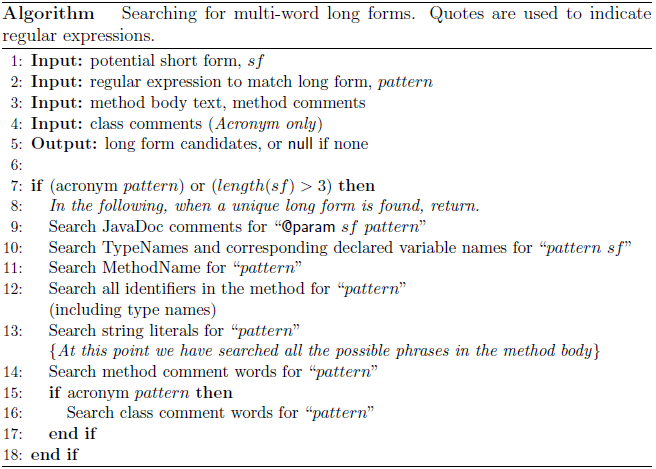
\includegraphics[scale=0.7]{./exp_2.png}
\caption{Algoritmo de Expansión Multi-Palabra.}
\label{exp2}
\end{figure}

El algoritmo presentado en la figura \ref{exp2} de búsqueda por multi-palabras\cite{EZH08} en la línea 6 se asegura de filtrar combinaciones de palabras largas incorrectas. Los patrones de \textit{combinación de palabras} son menos restrictivos que los patrones de \textit{acrónimos} y frecuentemente conllevan a malas decisiones. La búsqueda se restringe a palabras abreviadas ingresadas con longitud 4 ó mayor. Esto genera la sensación de que se pierden casos de 2 ó 3 caracteres pero estudios indican que son la minoría\cite{EZH08}.
 
Al igual que el algoritmo anterior en las líneas 8-10 se realiza la búsqueda primero en comentarios JAVA Doc, luego en nombres de tipos, después en nombres de los métodos (Figura \ref{exp3}). Dado que la complejidad de tiempo tiene cotas altas cuando se busca con expresiones regulares multi-palabras en sentencias, esta búsqueda no se realiza como se hizo en el algoritmo anterior. En las siguientes líneas 11-13 se examinan los ids(incluyendo declaraciones), literales strings y comentarios del método. Finalmente en la línea 15 se busca en comentarios de la clase con el patrón acrónimo. Cabe aclarar que al igual que el \textit{patrón compuesto por letras} en el algoritmo anterior, el \textit{patrón de combinación de palabras} en este caso no se usa ya que puede tomar palabras largas incorrectas.

Finalmente después de observar cientos de casos de palabras largas los autores concluyen que el mejor orden de ejecución de las técnicas de búsqueda es ejecutar los patrones: acrónimo, prefijo, compuesto por letras, combinación de palabras.

Si ninguna de las estrategias de expansión funciona en el ámbito local dentro de un método, se procede a buscar la palabra abreviada en un listado de contracciones mas comunes. Si finalmente sigue si poder encontrarse una coincidencia se recurre a la técnica conocida como expansión mas frecuente (MFE).\\

\noindent \textbf{Decidir entre Múltiples Alternativas\\}

Existe la posibilidad de que una abreviación posea múltiples alternativas potenciales de expansión dentro del mismo alcance estático. Por ejemplo el patrón prefijo para \textsf{val} puede coincidir \textsf{value} o \textsf{valid}. La técnica de elección entre múltiples candidatos procede de la siguiente manera:

\begin{enumerate}
\itemsep0em%reduce espacio
\item Se elije la palabra larga dentro del alcance estático con mayor frecuencia de aparición. Tomando el ejemplo anterior para \textsf{val} si \textsf{value} aparece 3 veces y \textsf{valid} una sola vez, se elije la primera.

\item Se agrupa las palabras largas con similares características. Por ejemplo si \textsf{def} coincide con \textsf{defaults}, \textsf{default} y \textsf{define} donde todas aparecen 2 veces, en este caso se agrupa las 2 primeras en solo \textsf{default} con una cantidad de 4 predominando sobre \textsf{define}.

\item En caso de que la igualdad persista, se acumulan las frecuencias de aparición entre las distintas búsquedas para determinar un solo candidato. Por ejemplo, si el id \textsf{fs} coincide con \textsf{file system} y \textsf{file socket} ambas con 2 apariciones en los comentarios de JAVA Doc, si en la búsquedas siguientes nombres de tipos de ids, literales, comentarios aparece \textsf{file socket} este termina prevaleciendo sobre \textsf{file system}.

\item Finalmente si todas las anteriores fallan se recurre al método de expansión mas frecuente (MFE). 

\end{enumerate}

\pagebreak
\noindent \textbf{Expansión Más Frecuente (MFE)\\}

La estrategia MFE\cite{EZH08} mejora la precisión de acertar con la expansión de una abreviatura. La idea consiste en ejecutar la misma estrategia local de expansión de abreviaturas explicada anteriormente pero sobre el programa entero. Para cada palabra abreviada, se cuenta el numero de veces que esa palabra se le asigna una palabra larga candidata. Luego se calcula la frecuencia relativa de una palabra abreviada con respecto a cada palabra larga encontrada. La palabra larga con mayor frecuencia relativa se considera la expansión mas frecuente. Al final del proceso se agrupan las palabras largas potenciales en un listado de MFE.

Sin embargo suele pasar que la expansión mas probable es la incorrecta. Para evitar que suceda se considera a su vez que una palabra larga debe superar en su frecuencia relativa mas de la mitad (0.5) y también que una palabra abreviada tenga al menos 3 asignaciones de palabras largas candidatas en todo el programa.

La técnica MFE tiene 2 niveles, el primero es a nivel de programa y el otro mas general a nivel JAVA. El nivel de programa es ideal ya que expande las abreviaturas con palabras propias del dominio del problema. El nivel mas general se arma con la API de Java. En la tabla \ref{tab_mfe} se muestra algunos casos de frecuencias relativas mas altas de JAVA 5. En caso de que una palabra abreviada no obtenga un candidato de expansión MFE también puede entrenarse sobre una gran cantidad de programas JAVA para mejorar la precisión. A su vez también existe la posibilidad de armar una lista a mano para casos puntuales de expansión que no son de frecuente aparición. Otras soluciones propuestas son entrenar sobre documentación online relacionada a JAVA o documentación vinculada a la ciencias de computación en general.

\begin{table}
\begin{center}
   \begin{tabular}{| l |l | l |}
     \hline \textsf{Abreviatura} & \textsf{Palabra Exp.} & \textsf{Frec. Relativa} \\
     \hline \textsf{int} & \textsf{integer} & 0.821 \\
     \hline \textsf{impl} & \textsf{implement} & 0.840 \\
     \hline \textsf{obj} & \textsf{object} & 1.000 \\
     \hline \textsf{pos} & \textsf{position} & 0.828 \\
     \hline	   
   \end{tabular}
   \label{tab_mfe}
\caption{Algunas Frecuencias Relativas de ids en JAVA 5}
\end{center}   
\end {table}


Este algoritmo de expansión de abreviaturas es totalmente automatizado y se implementó como un plugin de Eclipse. Actualmente solo soporta procesamiento por lotes pero se tiene pensado que corra en segundo plano brindando apoyo a herramientas de mantenimiento de software\cite{EZH08}.\\

%Extracting meaning - lawrie
Hasta ahora se han descripto algoritmos y técnicas que recientemente se pensaron y elaboraron. En la próxima sección se presenta una herramienta que fue construida en los comienzos de los estudios basados en ids. La herramienta se encarga de hacer una reestructuración de nombres de ids y es tomada como objeto de estudio por varios autores\cite{EZH08,DCHD06,DLHD06,LFBEX07}.



%tonella-caprile
\pagebreak 
\subsection{Herramienta: Identifier Restructuring}

\begin{figure}[h] %[h] para here [b] para bottom [t] para top
\centering
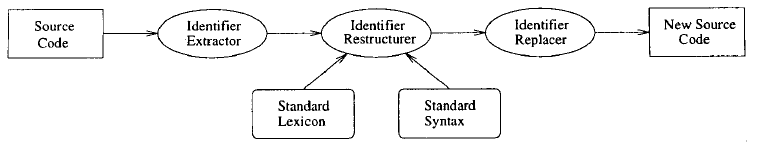
\includegraphics[scale= 0.80]{./ire_1.png}
\caption{Etapas de Restructuring tool}
\label{ire1}
\end{figure}

La herramienta Restructuring Tool\cite{BCPT00} se encarga de recibir como entrada un código fuente escrito en lenguaje C y luego a través de un proceso de transformación cada nombramiento de los ids(solo trabaja con ids del tipo hardword), se expande a palabras completas, retornando de esta manera el mismo código pero con los ids expandidos.

Los nombres se cambian por nombres mas explicativos agregando un verbo que indica la función del id en el código, mas precisamente después de renombrar los ids se visualiza claramente el rol que cumple el id en el programa.

El código fuente se convierte de esta manera en un código mas entendible y mejora la comprensión. El proceso consta de tres etapas (Figura \ref{ire1}): 

\begin{enumerate}
\itemsep0em%reduce espacio
\item \textbf{Identifier Extractor:} Recupera una lista con los nombres de los ids presentes en el código. Este módulo se programó con un parser modificado de C que reconoce los ids y los extrae.
\item \textbf{Identifier Restructurer:} Genera una asociación entre el nombramiento actual del id y un nuevo nombramiento estándar expandido. El primer paso consiste en segmentar el id en las palabras que lo constituyen, después cada palabra se expande usando un diccionario de palabras estándar (estándar léxico) y finalmente la secuencia de palabras del id debe coincidir con reglas predefinidas por una gramática para determinar que acción cumple el id en el código \mbox{(estándar sintáctico).}
\item \textbf{Identifier Replacer:} Transforma el código original en el nuevo código usando las asociaciones que se construyeron en la etapa anterior. Se emplea un scanner léxico para evitar reemplazar posibles nombres de ids contenidos en literales strings y en comentarios.
\end{enumerate}

Los pasos 1 y 3 están totalmente automatizados. Sin embargo no sucede lo mismo con el paso 2 porque se necesita la intervención del programador para lograr una expansión adecuada de nombres.

\begin{figure}[h] %[h] para here [b] para bottom [t] para top
\centering
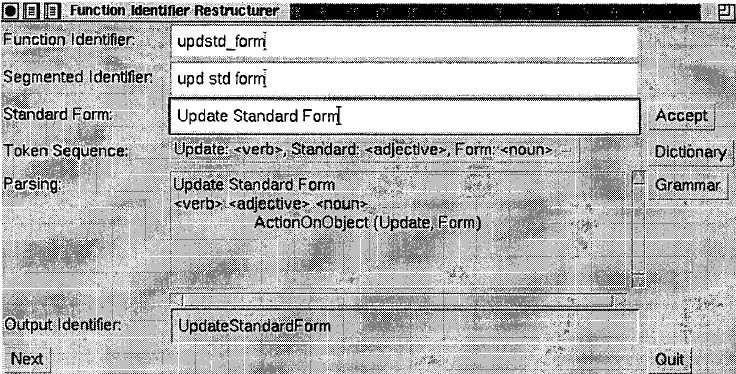
\includegraphics[scale= 0.60]{./ire_2.png}
\caption{Etapas en la transformación del id.}
\label{ire2}
\end{figure}

\begin{figure}[t] %[h] para here [b] para bottom [t] para top
\centering
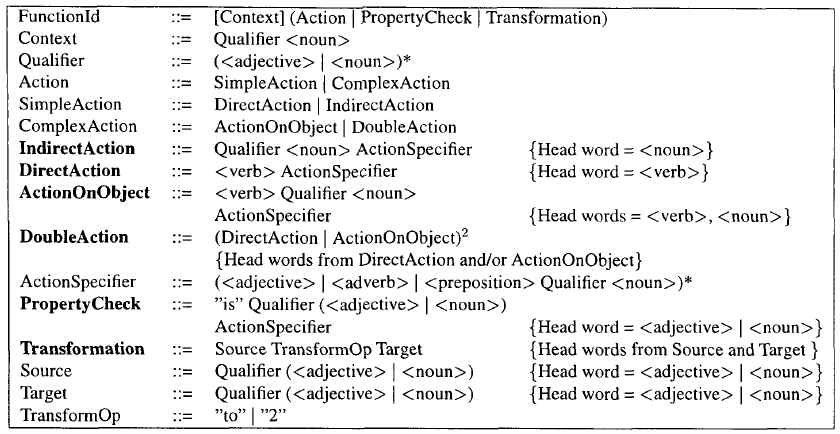
\includegraphics[scale= 0.70]{./ire_3.png}
\caption{Gramática que determina la función de los ids.}
\label{ire3}
\end{figure}

A continuación se detalla el paso 2 que es el mas importante de esta herramienta, en la Figura \ref{ire2} se desglosa las diferentes etapas.

\begin{description}
\itemsep0em%reduce espacio
\item[Segmentation:] El id es separado en las palabras que lo componen. De manera automática se utilizan estrategias de separación (basada en guion bajo o camel-case: hardword) en caso de no hacer correctamente la división el usuario puede hacer de forma manual. A nivel conceptual (no implementado) se usa un diccionario para reconocer cada palabra del id. Un algoritmo hecho en LISP toma un string \textit{s} como entrada, utiliza una estrategia greedy verificando a partir de la primer letra de \textit{s} un sub-string que pertenezca en el diccionario, luego el sub-string se descarta y continua el análisis con el resto hasta que no haya mas sub-strings que separar\cite{BCPT99}.

\item[Standard Lexicon:] Una vez lograda la separación de las palabras estas son mapeadas a una forma estándar(expandidas) con la ayuda de un diccionario léxico\cite{BCPT99}(Ejemplo: \textsf{upd} $\rightarrow$ \textsf{Update}). Este diccionario puede ser definido por el usuario al igual que el procedimiento para actualizarlo. En caso de que no exista una asociación se puede construir un diccionario de sinónimos con términos extraídos del código fuente que se consideran estándares y sino el usuario puede realizar la expansión manualmente. Para comenzar el análisis los autores\cite{BCPT00} de la herramienta construyeron los diccionarios de manera genérica tomando como muestra 10 programas. Sin embargo se aconseja que con el tiempo los diccionarios deben crecer con la inclusión de nuevos términos.

\item[Tokenization:] Una vez obtenidas las palabras a una forma estándar en el paso anterior, se procede a asignar cada palabra a un \textit{tipo léxico} (verbo, sustantivo, adjetivo). Por ejemplo la palabra Update $\rightarrow$ $<$Update,verb$>$ y Standard $\rightarrow$ $<$Standard,adjective$>$. Esta tuplas se denominan tokens y se utiliza un `diccionario de tipos' para generarlos de manera automática, este diccionario al igual que los otros se arma previamente a gusto del programador\cite{BCPT99}. Sin embargo existen casos que se necesita la intervención humana para determinar el tipo correcto, por ejemplo: free en inglés es un verbo, es un adjetivo y a la vez un adverbio.% En este caso la herramienta va a elegir lo que el diccionario le indique (si free esta presente).

\item[Parsing:] Finalmente la secuencia de tokens obtenidos en la etapa anterior se parsea usando una gramática predefinida para determinar cual es el rol/acción del id en el código fuente y de esta manera se determina la `acción semántica' del id. Esta gramática puede ser construida por el usuario, en la figura \ref{ire3} se muestra la desarrollada por los autores. Es una gramática regular donde los símbolos terminales están indicados con $<>$, las producciones con negrita indican distintos tipos de ids donde el verbo expresa la acción y el sustantivo representa al objeto de la acción, por ejemplo \textbf{ActionOnObject} $\Rightarrow$ $<$verb$>$,$<$noun$>$ $\equiv$ $<$go,home$>$ por ejemplo.

En caso de que el parseo falle el proceso se reinicia desde el comienzo partiendo nuevamente de la etapa de segmentación\cite{BCPT00} (figura \ref{ire2}).
\end{description}

\begin{figure}[t] %[h] para here [b] para bottom [t] para top
\centering
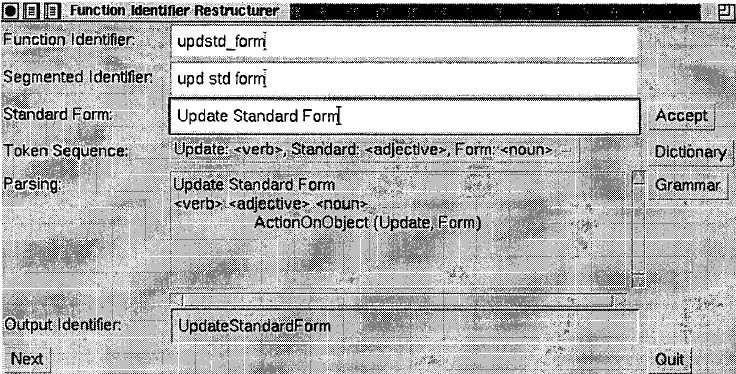
\includegraphics[scale= 0.80]{./ire_4.png}
\caption{Visualización de Restructuring Tool.}
\label{ire4}
\end{figure}

La interfaz de usuario de \textbf{Identifier Restructurer} se visualiza en la figura \ref{ire4}, el id de entrada se muestra en el primer cuadro de texto \textsf{updstd\_form}. Se usa heurísticas sencillas(guión bajo, camel-case) para separar las palabras del id, en este caso \textsf{updstd} y \textsf{form}. Como esta segmentación esta incompleta el usuario puede separar manualmente en el segundo cuadro de texto la palabra \textsf{upd} y \textsf{std}. En el tercer cuadro de texto se propone la forma estándar de cada palabra. Cuando una palabra no se puede expandir la herramienta muestra un signo de pregunta en su lugar (?). En este caso \textsf{upd} $\rightarrow$ \textsf{Update}, \textsf{std} $\rightarrow$ (?), \textsf{form} $\rightarrow$ \textsf{Form}, como \textsf{std} no esta presente en el diccionario se necesita la intervención del desarrollador para que se complete correctamente a \textsf{Standard}. Luego las palabras expandidas son asociadas a la función gramatical. En esta etapa puede existir para una secuencia de palabras mas de una función gramatical(la gramática es ambigua y puede generar mas de una secuencia de tokens). En caso de suceder esto el usuario puede elegir cual es la secuencia mas adecuada. En el ejemplo mostrado solo existe una única función gramatical y es reflejada en el cuarto cuadro de texto(figura \ref{ire4}). Luego en el cuadro de Parsing se puede apreciar la acción que aplica el id, en este caso \textbf{ActionOnObject(Update,Form)} `actualizar formulario'. Finalmente el resultado se detalla en el último cuadro de texto de mas abajo.

Cuando se arma la asociación de los nombres ids con los nuevos nombres generados la misma debería cumplir con la propiedad de inyectividad, de esta forma se evita que haya conflictos de nombres entre los distintos ids del programa. Al final de esta etapa la herramienta ayuda al programador a conseguir este objetivo resaltando los posibles conflictos en los nombres.

Para concluir la etapa \textbf{Identifier Replacer} toma todas las ocurrencias del id \textsf{updstd\_form} y se reemplaza por \textsf{UpdateStandarForm}, como se mencionó con anterioridad.

\section{Conclusiones}

Las observaciones que se destacan en el estado del arte de las técnicas de análisis de ids apuntan al nombramiento correcto de los ids. Al comienzo de este capitulo se detalló una herramienta que ayuda a lograr esta meta, sin embargo no trascendió ya que es costosa de utilizar sobre grandes proyectos de software y solo es efectiva cuando se emplea desde el arranque del desarrollo de un sistema.

El correcto nombramiento en los ids es crucial para la comprensión de los sistemas. Además en este contexto se facilitan las tareas que realizan las herramientas/técnicas encargadas de extraer conceptos del dominio del problema basándose en ids. 

Estas herramientas/técnicas han ido evolucionando con el pasar del tiempo. Al principio algunas etapas necesitaban la intervención del usuario para realizar las tareas, se puede decir entonces que usaban procesos semi-automatizados. A medida que se construyeron nuevas técnicas, se buscó más la automatización haciendo que el programador se involucre menos.

Como se mencionó en este capítulo, las primeras técnicas utilizaban netamente diccionarios de palabras en lenguaje natural, lo cual requiere mucho espacio de almacenamiento. Mas tarde se intentó disminuir el uso de estos diccionarios mirando más los recursos internos de información dentro los sistemas, como es el caso de los comentarios, literales strings y la documentación.

Sin embargo, suele ocurrir que estos recursos internos son escasos, entonces los autores de las recientes técnicas decidieron recurrir a procesos que examinan programas de gran envergadura y recolectar palabras útiles que ayuden a traducir el significado de los ids en los códigos. De esta forma se dispone de diccionarios con bajas exigencias de almacenamiento y que están constituidos de palabras mas adecuadas al ámbito de las ciencias de la computación.


%Con este estudio se puede observar que los ids son una fuente importante de información, por eso elaborar técnicas que analicen ids es un aporte destacado para la CP.

%\section{Técnicas de División de Identificadores}
%\section{Técnicas de Expansión de Identificadores}

%En el área de Ingeniería del Software, existen herramientas automatizadas que permiten hacer análisis de los identificadores utilizados en los códigos de programación. Estas herramientas extraen parcialmente conceptos representados en los identificadores del código fuente para intentar interpretar lo que el programador quiso desarrollar.

%Estas técnicas exhiben información estática oculta detrás de los ids, esta información es importante porque da indicios de lo que un sistema realiza en su ejecución por ende es un aporte en el ámbito de Comprensión de Programas. --colocar abajo

%========================================================================
\bibliographystyle{plain}%{alpha}
\bibliography{biblo.bib}

\end{document}
